
\documentclass{article}  % sysml

\usepackage{booktabs}
\usepackage{hyperref}
\newcommand{\theHalgorithm}{\arabic{algorithm}}
% \usepackage[accepted]{sysml2019}
\usepackage[accepted]{mlsys2020}
% \usepackage{sysml2019}


\newcommand{\npapers}{\text{81 }}
\newcommand{\rawnpapers}{81}

% \usepackage{flafter}  %

% \usepackage[sorting=ynt]{biblatex}
% \usepackage[sorting=ynt]{natbib}
% \usepackage[sort]{natbib}
% \DeclareSortingScheme{noneyear}{
%  \sort{\citeorder}
%  \sort{\field{year}}
% }

% \usepackage[sorting=ynt]{natbib}

%-------------------------------------------------------------- Includes

\usepackage{bbm}  % who knows?

\usepackage{amsmath}          % basic math
\usepackage{amssymb} 			    % math symbols
% \usepackage{amsthm}           % theorems
\usepackage{textcomp}

% \usepackage{float}            % make figures work
% \usepackage{cite}             % citations would be nice
\usepackage{url}              % better urls; magically keeping doc from breaking due to urls in refs

% \usepackage{tabu}
\usepackage{array}            % multiline table cells; somehow
\usepackage{tabularx}         % better tables
% \usepackage[table]{xcolor}    % colored table cells  % incompatible with sigconf
\usepackage{colortbl}
\newcolumntype{Y}{>{\centering\arraybackslash}X}	% centered column type for tabularx

% stuff for piecewise functions
\usepackage{mathtools}          %loads amsmath as well
\DeclarePairedDelimiter\Floor\lfloor\rfloor
\DeclarePairedDelimiter\Ceil\lceil\rceil

% \DeclareMathOperator*{\argmin}{arg\,min} % argmin
% \DeclareMathOperator*{\argmax}{arg\,max} % argmax
\DeclareMathOperator*{\argmin}{argmin} % argmin
\DeclareMathOperator*{\argmax}{argmax} % argmax

\usepackage{pbox}   % for trick to force linebreaks in table cells

\usepackage{setspace}
% \usepackage{setspace}

% \usepackage{booktabs} % acm recommended, and for pandas latex tables

%-------------------------------------------------------------- Algorithm setup

% commented out for sysml

% \usepackage{algorithm}
% \usepackage[noend]{algpseudocode} % I think this removes trailing "end {if,for,while}"

% % \algnewcommand{\LineComment}[1]{\State \(\triangleright\) #1} % left-aligned comments
% % \algnewcommand{\SideComment}[1]{\(//\) #1}
% \algnewcommand{\COMMENT}[2][.5\linewidth]{\leavevmode\hfill\makebox[#1][l]{//~#2}}
% \algnewcommand{\LineComment}[1]{\State \(//\) #1}	% left-aligned comments
% \algnewcommand\RETURN{\State \textbf{return} }


%-------------------------------------------------------------- Figures setup

% \usepackage[pdftex]{graphicx}
\usepackage{graphicx}
\usepackage[space]{grffile}   % allow spaces in file names
% declare the path(s) where your graphic files are
% \graphicspath{{../figs/survey/}}
\graphicspath{{./figs/}}
% and their extensions so you won't have to specify these
\DeclareGraphicsExtensions{.pdf,.jpeg,.jpg,.png}


%\textfloatsep: space between last top float or first bottom float and the text (default = 20.0pt plus 2.0pt minus 4.0pt).
%\intextsep : space left on top and bottom of an in-text float (default = 12.0pt plus 2.0pt minus 2.0pt).
\setlength{\textfloatsep}{4pt}
\setlength{\intextsep}{4pt}

% \usepackage{caption}
% \usepackage[font={small,it}]{caption}
\usepackage[font={bf}]{caption}
\setlength{\abovecaptionskip}{1pt} % less space between captions and figures
% \setlength{\abovecaptionskip}{-2pt} % less space between captions and figures
% \setlength{\abovecaptionskip}{-5pt}	% less space between captions and figures
% \setlength{\belowcaptionskip}{-13pt}  % less space below captions
% \setlength{\belowcaptionskip}{-10pt}  % less space below captions
\setlength{\belowcaptionskip}{-4pt}	% less space below captions

% \usepackage{paralist}
% \setdefaultleftmargin{10pt}{10pt}{}{}{}{}

% \usepackage{changepage}
% \usepackage{tabulary}

\usepackage{outlines}
\usepackage{enumitem}
\newcommand{\ItemSpacing}{0mm}
\newcommand{\ParSpacing}{0mm}
\setenumerate[1]{itemsep={\ItemSpacing},parsep={\ParSpacing},label=\arabic*.}
% \setenumerate[2]{itemsep={\ItemSpacing},parsep={\ParSpacing},label=\arabic*.}
\setenumerate[2]{itemsep={\ItemSpacing},parsep={\ParSpacing}}

% \usepackage[linewidth=1pt]{mdframed}
% \mdfsetup{frametitlealignment=\center, skipabove=0, innertopmargin=1mm,
% innerleftmargin=2mm, leftmargin=0mm, rightmargin=0mm}

%-------------------------------------------------------------- Miscellaneous setup

% \usepackage{enumitem}
% \setlist{nolistsep}
% \setlist{first=itemsep1em}
% \setlist[1]{labelindent=\parindent}

% \newlength\myindent
% \setlength\myindent{2em}
% \newcommand\bindent{%
%   \begingroup
%   \setlength{\itemindent}{\myindent}
%   \addtolength{\algorithmicindent}{\myindent}
% }
% \newcommand\eindent{\endgroup}

% remove unwanted space between paragraphs;
% it's set by the IEEE conference format, but no papers from this conference have it
% \parskip 0ex plus 0.2ex minus 0.1ex

% make vectors be bold instead of with arrows
\renewcommand{\vec}[1]{\mathbf{#1}}
% add 'mat' command to make matrices bold
\newcommand{\mat}[1]{\mathbf{#1}}

\DeclarePairedDelimiter\ceil{\lceil}{\rceil}
\DeclarePairedDelimiter\floor{\lfloor}{\rfloor}

\newtheorem{Definition}{Definition}[section]

% ------------------------ convenience commands
\newcommand\eps\varepsilon
\DeclareMathOperator{\infimum}{inf}
\renewcommand\inf\infty
\DeclareMathOperator{\erfc}{erfc}

\renewcommand{\c}{\vec{c}}
\newcommand{\q}{\vec{q}}
\renewcommand{\r}{\vec{r}}
\renewcommand{\v}{\vec{v}}
\newcommand{\vhat}{\hat{\vec{v}}}
\newcommand{\x}{\vec{x}}
\newcommand{\xhat}{\hat{\vec{x}}}
\newcommand{\y}{\vec{y}}
\newcommand{\yhat}{\hat{\vec{y}}}
\newcommand{\z}{\vec{z}}
\newcommand{\zhat}{\hat{\vec{z}}}

\newcommand{\lam}{\lambda}
\newcommand{\sig}{\sigma}
\newcommand{\Sig}{\Sigma}

\newcommand{\E}{\mathop{{}\mathbb{E}}}

\renewcommand{\H}{\mathcal{H}}
\newcommand{\R}{\mathbb{R}}
\newcommand{\V}{\mathcal{V}}
\newcommand{\Xs}{\mathcal{X}}
\newcommand{\Z}{\mathcal{Z}}
\renewcommand{\S}{\mathcal{S}}
\newcommand{\Nb}{\mathcal{N}_b}

\newcommand{\onehalf}{\frac{1}{2}}

\newcommand{\Xcal}{\mathcal{X}}
\newcommand{\Ycal}{\mathcal{Y}}

\newcommand{\pie}[1]{\frac{\pi}{#1}}
% \newcommand{\pitwo}{\frac{\pi}{2}}
% \newcommand{\pifour}{\frac{\pi}{4}}

% \newcommand{\norm}[1]{\left\lVert #1 \right\rVert}
\DeclarePairedDelimiter\abs{\lvert}{\rvert}%
\DeclarePairedDelimiter\norm{\lVert}{\rVert}%

\DeclareMathOperator{\Beta}{Beta}
\DeclareMathOperator{\Normal}{\mathcal{N}}
\DeclareMathOperator{\erf}{erf}
\DeclareMathOperator{\Var}{Var}

% make *all* text 10pt
% \renewcommand{\footnotesize}{\normalsize}
% \renewcommand{\footnotesize}{\small}
% \renewcommand{\small}{\normalsize}

% ------------------------------------------------ stuff that might break things


% \usepackage{mathtools}
% \usepackage{amsthm}           % theorems
% \newtheorem{theorem}{Theorem}[section]
% \newtheorem{lemma}{Lemma}[section]
% \newtheorem{definition}{Definition}[section]
% \newtheorem{corollary}{Corrolary}[section]


% optional custom title for header
% \sysmltitlerunning{What is the State of Neural Network Pruning?}
\mlsystitlerunning{What is the State of Neural Network Pruning?}

\begin{document}

\twocolumn[
% ================================================================
\mlsystitle{What is the State of Neural Network Pruning?}
% \mlsystitle{Have We Actually Learned Anything about Pruning Neural Networks?}

\mlsyssetsymbol{equal}{*}
\begin{mlsysauthorlist}
\mlsysauthor{Davis Blalock}{equal,csail}
\mlsysauthor{Jose Javier Gonzalez Ortiz}{equal,csail}
\mlsysauthor{Jonathan Frankle}{csail}
\mlsysauthor{John Guttag}{csail}
\end{mlsysauthorlist}

\mlsysaffiliation{csail}{MIT CSAIL, Cambridge, MA, USA}
\mlsyscorrespondingauthor{Davis Blalock}{dblalock@mit.edu}

% apparently these only show up in pdf metadata, not document
\mlsyskeywords{Deep Learning, Pruning}

% \vskip 0.3in
\vskip 0.2in

% ------------------------------------------------
\begin{abstract}
% ------------------------------------------------

Neural network pruning---the task of reducing the size of a network by removing parameters---has been the subject of a great deal of work in recent years. We provide a meta-analysis of the literature, including an overview of approaches to pruning and consistent findings in the literature. After aggregating results across \npapers papers and pruning hundreds of models in controlled conditions, our clearest finding is that the community suffers from a lack of standardized benchmarks and metrics.
This deficiency is substantial enough that it is hard to compare pruning techniques to one another or determine how much progress the field has made over the past three decades.
To address this situation, we identify issues with current practices, suggest concrete remedies, and introduce ShrinkBench, an open-source framework to facilitate standardized evaluations of pruning methods. We use ShrinkBench to compare various pruning techniques and show that its comprehensive evaluation can prevent common pitfalls when comparing pruning methods.

\end{abstract}
]  % end of manual twocolumn for sysml

% \maketitle

\printAffiliationsAndNotice{\mlsysEqualContribution} % otherwise use the standard text.

% ================================================================
\section{Introduction} \label{sec:intro}
% ================================================================
\vspace{-.75mm}

\section{Introduction}
\label{sec:intro}

% \begin{itemize}
%     \item Generic intro for deep speaker embeddings incl x-vectors
%     \item How are x-vectors used in speaker diar? AHC+PLDA, k-means, SC
%     \item How are x-vectors used in SV?
%     \item Reformulation as multiple tasks
%     \begin{itemize}
%             \item Although it works so well, current setup is single-task which transfer learns embeddings for unseen classes
%             \item By randomly sampling a subset of classes during training, we can easily formulate as multiple related tasks
%             \item Meta-learning generalizes across multiple tasks, hence a natural choice here
%     \end{itemize}
%     \item Contributions
%     \begin{itemize}
%         \item Generic speaker embeddings trained using meta-learning objectives, unlike prev works which focused on one
%         \item \textbf{(Pending results)} Application of relation networks for speaker embedding training (or) combining deep clustering with meta learning
%         \item Open-source toolkit for reproducible research
%     \end{itemize}
% \end{itemize}

Audio speaker embeddings refer to fixed-dimensional vector representations extracted from variable duration audio utterances and assumed to contain information relevant to speaker characteristics. In the last decade, speaker embeddings have emerged as the most common representations used for speaker-identity relevant tasks such as speaker diarization (speaker segmentation followed by clustering: \textit{who spoke when?}) \cite{anguera_DiarOverview2012} and speaker verification \textit{(does an utterance pair belong to same speaker?}) \cite{campbell_speakerRecogTutorial1997}.
Such applications are relevant across a variety of domains such as 
voice bio-metrics \cite{rahulamathavan_bioMetrics2019, scheffer_bioMetrics2013}, automated meeting analysis \cite{anguera2007acoustic,vanLeeuwen_meeting2006}, and clinical interaction analysis \cite{pal_clusterGAN2020, xiao2016technology}. Recent technology evaluation challenges \cite{ryant2019second, richey2018voices, Hansen_fearlessSteps2018, McLaren_SITW2016} have drawn attention to these domains by incorporating natural and simulated in-the-wild speech corpora exemplifying the many diverse technical facets that need to be addressed. 

While initial efforts toward training speaker embeddings had focused on generative modeling \cite{reynolds2000speaker,campbell_SVMGMM2006} and factor analysis \cite{dehak_ivectors2011}, deep neural network (DNN) representations extracted at bottleneck layers have become the standard choice in recent works. The most widely used representations are trained using a classification loss (d-vectors \cite{origdvec_variani2014deep}, x-vectors \cite{snyder_xvec2017, snyder_xvec2018}), while other training objectives such as triplet loss \cite{bredin_tristounet2017, zhang_triplet2018} and contrastive loss \cite{chung2018Voxceleb2} have also been explored.
%Following training, the output layer is removed and bottleneck representations are treated as speaker embeddings.
More recently, end-to-end training strategies \cite{Fujita2019, horiguchi2020endtoend, fujita2020endtoend} have been proposed for speaker diarization to address the mismatch between training objective (classification) and test setup (clustering, speaker selection, etc).

A common factor in the classification formulation is that all the speakers from training corpora are used throughout the training process for the purpose of loss computation and minimization. Typically, categorical cross-entropy is used as the loss function.
While the number of speakers (classes) can often be large in practice ($\mathcal{O}(10^3)$), the classification objective represents a single task, i.e., the same speaker set is used to minimize cross-entropy at every training minibatch.
This entails limited task diversity during the training process and offers scope for training better speaker-discriminative embeddings by introducing more tasks.
We note that a few approaches exist which introduce multiple objectives for embedding training, such as metric-learning with cross entropy \cite{XU2020394, ren2019} and speaker classification with domain adversarial learning \cite{zhou2019dann, wang2018dann}. While these approaches demonstrate improvements over a single training objective, the speaker set is often common across objectives (except in domain adversarial training where target speaker labels are assumed unavailable).
% \textbf{TO ADD: Check comments in source file}\\
% Contrast this work with multiple loss functions during training:
% 1. https://www.sciencedirect.com/science/article/pii/S092523122031016X
% 2. Combining CE with triplet: https://arxiv.org/pdf/1908.02283.pdf
% So-called multi-task frameworks esp in adversarial training: Here, mention that "task" in these works refers to the objective itself, like CE, triplet, etc
% 3. https://ieeexplore.ieee.org/stamp/stamp.jsp?tp=&arnumber=8683828 
% Check with Taejin about continual learning with replays for speaker embedding training

In this work we use the classification framework while training neural speaker embeddings, however we decompose the original classification task into multiple tasks wherein each training step optimizes on a new task. 
A common encoder is learnt over this ensemble of tasks and used for extracting speaker embeddings during inference.
At each step of speaker embedding training, we construct a new task by sampling speakers from the training corpus. For a large training speaker set available in typical training corpora,
generating speaker subsets results in a large number of tasks.
%sampling results in a factorially (right term?) large number of tasks. 
This provides a natural regularization to prevent task over-fitting. 
Our approach is inspired by the meta-learning \cite{Schmidhuber_thesis} paradigm, also known as {\it learning to learn}. Meta-learning optimizes at two-levels: within each task and across a distribution of tasks \cite{ravi2017}. This is in contrast to conventional supervised learning which optimizes a single task over a distribution of samples. 
In addition to benefits from increased task variability meta-learning has demonstrated success in unseen classes \cite{ravi2017, finn_maml2017,Andrychowicz_2016}.
This forms a natural fit for applications such as speaker diarization and speaker verification which often evaluate on speakers unseen during embedding training.

We compare our meta-learned models with x-vectors, which have established state-of-the-art performance in multiple applications \cite{snyder_xvec2017, snyder_xvec2018} including recent evaluation challenges such as DIHARD\cite{Sell2018_dihard} and VOiCES \cite{richey2018voices}. 
First, we develop a competitive wide-band x-vector baseline using the PyTorch toolkit (calibrated with identical performance with the Kaldi Voxceleb recipe\footnote{https://github.com/kaldi-asr/kaldi/tree/master/egs/voxceleb}). 
Next, we use two different metric-learning objectives to meta-learn the speaker embeddings: prototypical networks and relation networks. While both approaches share the task sampling strategy during the training phase, they differ in the choice of the comparison metric between samples. We evaluate our approaches on two different applications: speaker diarization and speaker verification to illustrate the generalized speaker discriminability nature of meta-learned embeddings. 
% Can expand on this after completing experiments?

The contributions of this work are as follows: we develop new speaker embeddings using meta-learning that are not restricted to an application.
Within each application, we demonstrate improvements using multiple corpora obtained under controlled as well as naturalistic speech interaction settings.
Furthermore, we identify conditions where meta-learning demonstrates benefits over conventional cross-entropy paradigm. 
We analyze diarization performance across different domains in the DIHARD corpora. We also consider the special case of impact of child age groups using internal child-adult interaction corpora from the Autism domain. We study the effect of data collection setups (near-field, far-field and obstructed microphones) and the level of degradation artifacts on the speaker verification performance.
While we present results using prototypical networks and relation networks, the proposed framework is independent of the specific metric-learning approach and hence offers scope for incorporating non-classification objectives such as clustering. It should be noted however that the application of relation networks has not been explored in speaker embedding research.
Finally, we present an open source implementation of our work, including x-vectors baselines, based on a generic machine learning toolkit (PyTorch)\footnote{https://github.com/manojpamk/pytorch\_xvectors}.











%================================================================
\section{Overview of Pruning}
%================================================================

% 

\documentclass{standalone}

% uncomment to preview:

% \usepackage{tikz}
% \usepackage{xcolor}
% \usetikzlibrary{
%     arrows.meta,
%     chains,
%     scopes,
%     positioning,
%     shapes.geometric
% }
% % layers
% \pgfdeclarelayer{background}
% \pgfdeclarelayer{foreground}
% \pgfsetlayers{background,main,foreground}

% \definecolor{baseColour}{RGB}{255, 128, 85}
% \definecolor{ncqColour}{RGB}{118, 165, 175}
% \definecolor{ncqColour2}{RGB}{162, 196, 201}

% % styles     
% \tikzset{
%     processDiagram/.style={
%         startstop/.style={
%             rectangle,
%             draw,
%             minimum width=3cm, 
%             minimum height=0.8cm,
%             join = by arrow,
%             fill = black!0,
%         },
%         decision/.style = {
%             diamond,
%             aspect=1.7,
%             draw,
%             minimum width=2.5cm, 
%             minimum height=1cm, 
%             align=center,
%             join = by arrow,
%             fill = black!0,
%         },
%         process/.style = {
%             rectangle, 
%             rounded corners, 
%             draw,
%             minimum width=3cm,
%             minimum height=0.8cm, 
%             align=center,
%             join = by arrow,
%             fill = black!0,
%         },
%         process2/.style = {
%             rectangle, 
%             rounded corners, 
%             draw,
%             minimum width=3cm,
%             minimum height=0.8cm, 
%             align=center,
%             join = by arrow,
%             fill = ncqColour2,
%         },
%         line/.style = {
%             -
%         },
%         invisible/.style = {
%             join = by line,
%             minimum width=0cm, 
%             minimum height=0cm,
%             inner sep=0pt,
%         },
%         invisititle/.style ={
%             font = \bfseries,
%             join = by arrow,
%             outer sep = 5pt,
%         },
%         title/.style = {
%             font = \bfseries,
%             fill = black!20,
%             join = by arrow,
%             minimum width = 3cm,
%             minimum height=0.8cm,
%             draw,
%         },
%         output/.style ={
%             join = by line,
%             minimum width=0cm, 
%             minimum height=0cm,
%             inner sep=0pt,
%             font = \itshape,
%             align = center,
%         },
%         arrow/.style = {
%             ->
%         },
%     }
% }

\begin{document}


\begin{tikzpicture}[processDiagram, node distance=4mm and 5cm]

{ [start chain=trunk going below]
    \node [startstop, on chain] (n0) {Snippet};
    % \node[output, on chain](n0o) {
    %     ''consle.log('a');\\
    %     console.log(foo)"
    % };
    \node [process, on chain] (n1) {\textbf{1) Compile}};
    \node [decision, on chain] (errors) {Has Errors?};
    {[start branch = c going below]
        \node [output, on chain = going right, xshift=-4.5cm] (c0o) {Yes};
        \node [invisible, on chain = going above, yshift=3.63cm] (i0) {};
        \node [process, on chain = going right, xshift=-3.5cm] (c1) {\textbf{2) Targeted Fixes}};
        \node [decision, on chain] (errors2) {Has Errors?};
        {[start branch = cc going left]
            \node[output, on chain, xshift=4cm] {No};
            \node[invisible, on chain = going below, yshift=-4.3cm] (i1) {};
        }
        \node [output, on chain] (c1o) {Yes};
        \node [process, on chain = going below] (c2) {\textbf{3) TS Codefixes}};
        \node [decision, on chain] (errors3) {Has Errors?};
        {[start branch = cc going left]
            \node[output, on chain, xshift=4.4cm] {No};
            \node[invisible, on chain = going left, xshift=4.8cm] {};
        }
        \node [output, on chain] (c2o) {Yes};
        \node [process, on chain] (c3) {\textbf{4) Line Deletion}};
        \node [invisible, on chain, yshift=-0.2cm] (i2) {};
        \node [invisible, on chain = going left, xshift=-0.1cm] (i3) {};
    }
    \node [output, on chain] (n1o) {No};
    \node [startstop, on chain] (n2) {Done};
    \draw [arrow] (i1) -> (n2);
    \draw [arrow] (i3) -> (n2);
}

\begin{pgfonlayer}{background}
    \path (c1.west |- c1.north)+(-0.3,0.6) node (a) {};
    \path (c3.east |- c3.south)+(+0.3,-0.3) node (b) {};
    \path[fill=yellow!20,rounded corners, draw=black!50, dashed](a) rectangle (b); 

    \node[above of = c1, yshift=0.2cm]{Code Corrections};
\end{pgfonlayer}


\end{tikzpicture}

\end{document}
\renewcommand{\algorithmicrequire}{\textbf{Input:}}
\label{sec:overview}
Before proceeding, we first offer some background on neural network pruning and a high-level overview of how existing pruning methods typically work.

\subsection{Definitions}

We define a neural network \emph{architecture} as a function family $f(x; \cdot)$.
The architecture consists of the configuration of the network's parameters and the sets of operations it uses to produce outputs from inputs, including the arrangement of parameters into convolutions, activation functions, pooling, batch normalization, etc.
Example architectures include AlexNet and ResNet-56.
We define a neural network \emph{model} as a particular parameterization of an architecture, i.e., $f(x; W)$ for specific parameters $W$.
Neural network \emph{pruning} entails taking as input a model $f(x; W)$ and producing a new model $f(x; M \odot W')$. Here $W'$ is set of parameters that may be different from $W$, $M \in \{0, 1\}^{|W'|}$ is a binary mask that fixes certain parameters to $0$, and $\odot$ is the elementwise product operator.
In practice, rather than using an explicit mask, pruned parameters of $W$ are fixed to zero or removed entirely.

\subsection{High-Level Algorithm}

There are many methods of producing a pruned model $f(x; M \odot W')$ from an initially untrained model $f(x; W_0)$, where $W_0$ is sampled from an initialization distribution $\mathcal{D}$.
Nearly all neural network pruning strategies in our survey derive from Algorithm \ref{alg:prune-after-training} \cite{learning-both}.
In this algorithm, the network is first trained to convergence.
Afterwards, each parameter or structural element in the network is issued a score, and the network is pruned based on these scores.
Pruning reduces the accuracy of the network, so it is trained further (known as \emph{fine-tuning}) to recover.
The process of pruning and fine-tuning is often iterated several times, gradually reducing the network's size.

Many papers propose slight variations of this algorithm.
For example, some papers prune periodically during training \cite{google-state-of-sparsity} or even at initialization \cite{snip}.
Others modify the network to explicitly include additional parameters that encourage sparsity and serve as a basis for scoring the network after training \cite{sparse-variational-dropout}.

\begin{algorithm}[h]
\caption{Pruning and Fine-Tuning}
\label{alg:prune-after-training}
\begin{algorithmic}[1]
\REQUIRE $N$, the number of iterations of pruning, and \\ \hspace{1.5em}$X$, the dataset on which to train and fine-tune
    \STATE $W \gets initialize()$
    \STATE $W \gets trainToConvergence(f(X; W))$

    \STATE $M \gets 1^{|W|}$
    \FOR{$i$ \text{ }in $1$ to $N$}%
        \STATE $M \gets prune(M, score(W))$%
        \STATE $W \gets fineTune(f(X; M \odot W))$%
    \ENDFOR
    \STATE \textbf{return} $M, W$
\end{algorithmic}
\end{algorithm}

\subsection{Differences Betweeen Pruning Methods}

Within the framework of Algorithm \ref{alg:prune-after-training}, pruning methods vary primarily in their choices regarding sparsity structure, scoring, scheduling, and fine-tuning.

\textbf{Structure.} Some methods prune individual parameters (\emph{unstructured pruning}). Doing so produces a sparse neural network, which---although smaller in terms of parameter-count---may not be arranged in a fashion conducive to speedups using modern libraries and hardware.
Other methods consider parameters in groups (\emph{structured pruning}), removing entire neurons, filters, or channels to exploit hardware and software optimized for dense computation \cite{pruning-filters, channel-lasso-lstsq}.

\textbf{Scoring.}
It is common to score parameters based on their absolute values, trained importance coefficients, or contributions to network activations or gradients. %, or other measures of saliency.
Some pruning methods compare scores locally, pruning a fraction of the parameters with the lowest scores within each structural subcomponent of the network (e.g., layers) \cite{learning-both}.
Others consider scores globally, comparing scores to one another irrespective of the part of the network in which the parameter resides \cite{snip, lottery-ticket}.

% There are a range of techniques for scoring parameters.
% It is common to issue lower scores to parameters with lower magnitudes \cite{learning-both}.
% Other techniques consider activations, gradients, or saliency scores in combination with magnitudes.

\textbf{Scheduling.}
Pruning methods differ in the amount of the network to prune at each step.
Some methods prune all desired weights at once in a single step \cite{rethinking-net-pruning}.
Others prune a fixed fraction of the network iteratively over several steps \cite{learning-both} or vary the rate of pruning according to a more complex function \cite{google-state-of-sparsity}.

\textbf{Fine-tuning.}
For methods that involve fine-tuning, it is most common to continue to train the network using the trained weights from before pruning.
Alternative proposals include rewinding the network to  an earlier state \cite{lottery-ticket-followup} and reinitializing the network entirely \cite{rethinking-net-pruning}.
% \citet{rethinking-net-pruning} suggest that, when performing structured pruning, reinitializing the network weights before fine-tuning has no detrimental affect on the accuracy of the eventual network.

\subsection{Evaluating Pruning}

Pruning can accomplish many different goals, including reducing the storage footprint of the neural network, the computational cost of inference, the energy requirements of inference, etc.
Each of these goals favors different design choices and requires different evaluation metrics.
For example, when reducing the storage footprint of the network, all parameters can be treated equally, meaning one should evaluate the overall compression ratio achieved by pruning.
However, when reducing the computational cost of inference, different parameters may have different impacts.
For instance, in convolutional layers, filters applied to spatially larger inputs are associated with more computation than those applied to smaller inputs.
 % the amount of computation is linear with respect to the input size. Thus, given two convolutional filters pruned by the same amount, the one with a larger input size will lead to higher computational savings.

Regardless of the goal, pruning imposes a tradeoff between model efficiency and quality, with pruning increasing the former while (typically) decreasing the latter. This means that a pruning method is best characterized not by a single model it has pruned, but by a family of models corresponding to different points on the efficiency-quality curve.
To quantify efficiency, most papers report at least one of two metrics. The first is the number of multiply-adds (often referred to as FLOPs) required to perform inference with the pruned network. The second is the fraction of parameters pruned. To measure quality, nearly all papers report changes in Top-1 or Top-5 image classification accuracy.

As others have noted \cite{lempitsky-cp-decomp, perforated-cnns, bayesian-compression, sze-energy-aware, learning-both, samsung-vbmf-tucker, ssl, thinet-channel-norms, amc-automl-han}, these metrics are far from perfect. Parameter and FLOP counts are a loose proxy for real-world latency, throughout, memory usage, and power consumption. % In particular, despite many papers assuming otherwise, the number parameters has little bearing on memory of activations
Similarly, image classification is only one of the countless tasks to which neural networks have been applied. However, because the overwhelming majority of papers in our corpus focus on these metrics, our meta-analysis necessarily does as well.

% %For example, a single convolutional filter might contain nine parameters but be applied to repeatedly to every region of an activation map.
% To evaluate computational costs, many papers measure the number of multiply-adds (often referred to as FLOPs) required to perform inference with the pruned network.

% In practice, nearly all pruning papers measure the compression ratio or FLOP reduction achieved by pruning, so we focus on these metrics throughout the paper. However, we acknowledge (as do others \cite{bayesian-compression, sze-energy-aware, learning-both, samsung-vbmf-tucker}) that these metrics may not capture the performance considerations of running neural network inference on modern hardware.

% A crucial aspect of the pruning problem is that it usually requires optimizing a tradeoff between efficiency and quality;
% %That is, achieving a particular efficiency threshold may require removing parameters such that performance on the network's task declines.
% this means that, when comparing pruning methods, it is important to consider the entire pruning/quality tradeoff curve for different amounts of pruning.


%================================================================
\vspace{-2mm}
\section{Lessons from the Literature} \label{sec:lessons}
\vspace{-.5mm}
%================================================================

% \input{lessons.tex}
% Given the dismal state of inter-paper comparisons, can we learn \textit{anything} from the existing work on neural network pruning? Our meta-analysis reveals that the answer is yes. % In this section, we discuss general lessons, findings surrounding the recently introduced \textit{lottery ticket hypothesis}, and novel findings mined from our aggregated results.

After aggregating results from a corpus of \npapers papers, we identified a number of consistent findings. In this section, we provide an overview of our corpus and then discuss these findings.

% ------------------------------------------------
\vspace{-.75mm}
\subsection{Papers Used in Our Analysis}
\vspace{-.25mm}
% ------------------------------------------------

Our corpus consists of 79 pruning papers published since 2010 and two classic papers \cite{optimal-brain-damage, optimal-brain-surgeon} that have been compared to by a number of recent methods. We selected these papers by identifying popular papers in the literature and what cites them, systematically searching through conference proceedings, and tracing the directed graph of comparisons between pruning papers. This last procedure results in the property that, barring oversights on our part, there is no pruning paper in our corpus that compares to any pruning paper outside of our corpus. Additional details about our corpus and its construction can be found in Appendix~\ref{sec:corpus}.

% We selected the \npapers papers used in our analysis in the following way. First, we conducted an ad hoc literature search, finding widely cited papers introducing pruning methods and identifying other pruning papers that cited them using Google Scholar. We then went through the conference proceedings from the past year's NeurIPS, ICML, CVPR, ECCV, and ICLR and added all papers we identified as being about pruning. Finally, during the course of cataloging which papers compared to which others, we added to our corpus any pruning paper that at least one existing paper in our corpus purported to compare to. We included both published papers and unpublished ones of reasonable quality (typically on arXiv).
% In short, we included essentially every reasonable-quality paper introducing a method of pruning neural networks that we could find, taking care to capture the full directed graph of papers and comparisons between them.

% ------------------------------------------------
\vspace{-1mm}
\subsection{How Effective is Pruning?}
\vspace{-.25mm}
% ------------------------------------------------

One of the clearest findings about pruning is that it works. More precisely, there are various methods that can significantly compress models with little or no loss of accuracy. In fact, for small amounts of compression, pruning can sometimes \textit{increase} accuracy \cite{learning-both, spectral-pruning}. This basic finding has been replicated in a large fraction of the papers in our corpus. % Plus, it has been found in conditions that control for most lurking variables we have discussed, since authors can compare the same model using the same code before and after pruning.
% is present in even in the first generation of pruning papers \cite{early-brain-damage, optimal-brain-surgeon},

Along the same lines, it has been repeatedly shown that, at least for large amounts of pruning, many pruning methods outperform random pruning \cite{nisp, google-state-of-sparsity, lottery-ticket-followup, divnet, apple-pfa, channel-lasso-lstsq}. Interestingly, this does not always hold for small amounts of pruning \cite{lottery-transfer}. Similarly, pruning all layers uniformly tends to perform worse than intelligently allocating parameters to different layers \cite{google-state-of-sparsity, learning-both, pruning-filters, nvidia-taylor-pruning, thinet-channel-norms} or pruning globally \cite{snip, lottery-ticket}. Lastly, when holding the number of fine-tuning iterations constant, many methods produce pruned models that outperform retraining from scratch with the same sparsity pattern \cite{zhang-accel-very-deep, nisp, bayesian-compression, channel-lasso-lstsq, thinet-channel-norms, lottery-ticket} (at least with a large enough amount of pruning \cite{apple-pfa}). Retraining from scratch in this context means training a fresh, randomly-initialized model with all weights clamped to zero throughout training, except those that are nonzero in the pruned model.

Another consistent finding is that sparse models tend to outperform dense ones for a fixed number of parameters. \citet{snip-followup} show that increasing the nominal size of ResNet-20 on CIFAR-10 while sparsifying to hold the number of parameters constant decreases the error rate. \citet{wavernn} obtain a similar result for audio synthesis, as do \citet{openai-block-sparse} for a variety of additional tasks across various domains. Perhaps most compelling of all are the many results, including in Figure~\ref{fig:arch_vs_prune}, showing that pruned models can obtain higher accuracies than the original models from which they are derived. This demonstrates that sparse models can not only outperform dense counterparts with the same number of parameters, but sometimes dense models with even more parameters.

% ------------------------------------------------
\subsection{Pruning vs Architecture Changes}
% ------------------------------------------------

One current unknown about pruning is how effective it tends to be relative to simply using a more efficient architecture. These options are not mutually exclusive, but it may be useful in guiding one's research or development efforts to know which choice is likely to have the larger impact. Along similar lines, it is unclear how pruned models from different architectures compare to one another---i.e., to what extent does pruning offer similar benefits across architectures?
% \begin{figure}[t]
% \begin{center}
% 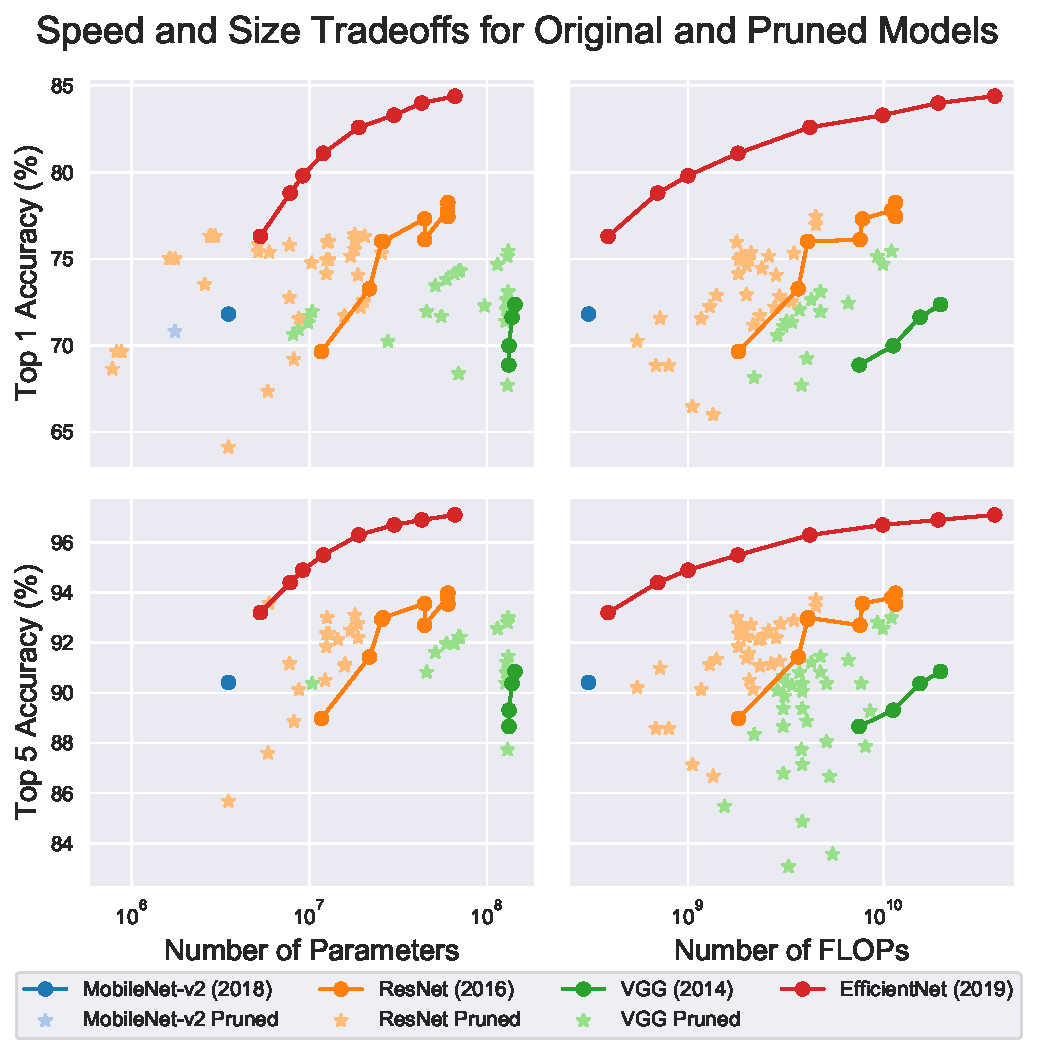
\includegraphics[width=\linewidth]{arch_vs_prune}
% \vspace{-3mm}
% \caption{Size and speed vs accuracy tradeoffs for different pruning methods and families of architectures. Pruned models sometimes outperform the original architecture, but rarely outperform a better architecture.}
% \label{fig:arch_vs_prune}
% \end{center}
% \end{figure}
To address these questions, we plotted the reported accuracies and compression/speedup levels of pruned models on ImageNet alongside the same metrics for different architectures with no pruning (Figure~\ref{fig:arch_vs_prune}).\footnote{
    Since many pruning papers report only change in accuracy or amount of pruning, without giving baseline numbers, we normalize all pruning results to have accuracies and model sizes/FLOPs as if they had begun with the same model. Concretely, this means multiplying the reported fraction of pruned size/FLOPs by a standardized initial value. This value is set to the median initial size or number of FLOPs reported for that architecture across all papers. This normalization scheme is not perfect, but does help control for different methods beginning with different baseline accuracies.
}
We plot results within a family of models as a single curve.\footnote{
    The EfficientNet family is given explicitly in the original paper \cite{efficientnet}, the ResNet family consists of ResNet-18, ResNet-34, ResNet-50, etc., and the VGG family consists of VGG-\{11, 13, 16, 19\}. There are no pruned EfficientNets since EfficientNet was published too recently. Results for non-pruned models are taken from \cite{efficientnet} and \cite{luigi}.
}

% We plot results within a family of models as a single curve. The EfficientNet family is given explicitly in the original paper \cite{efficientnet}, the ResNet family consists of ResNet-18, ResNet-34, ResNet-50, etc., and the VGG family consists of VGG-\{11, 13, 16, 19\}. There are no pruned EfficientNets since EfficientNet was published too recently. Results for non-pruned models are taken from \cite{efficientnet} and \cite{luigi}.

Figure~\ref{fig:arch_vs_prune} suggests several conclusions. First, it reinforces the conclusion that pruning can improve the time or space vs accuracy tradeoff of a given architecture, sometimes even increasing the accuracy. Second, it suggests that pruning generally does not help as much as switching to a better architecture. Finally, it suggests that pruning is more effective for architectures that are less efficient to begin with. % Finally, it suggests that pruning is more effective at reducing the size of models (left column) than their number of FLOPs (right column). This is unsurprising,

% \begin{figure}[t]
% \begin{center}
% 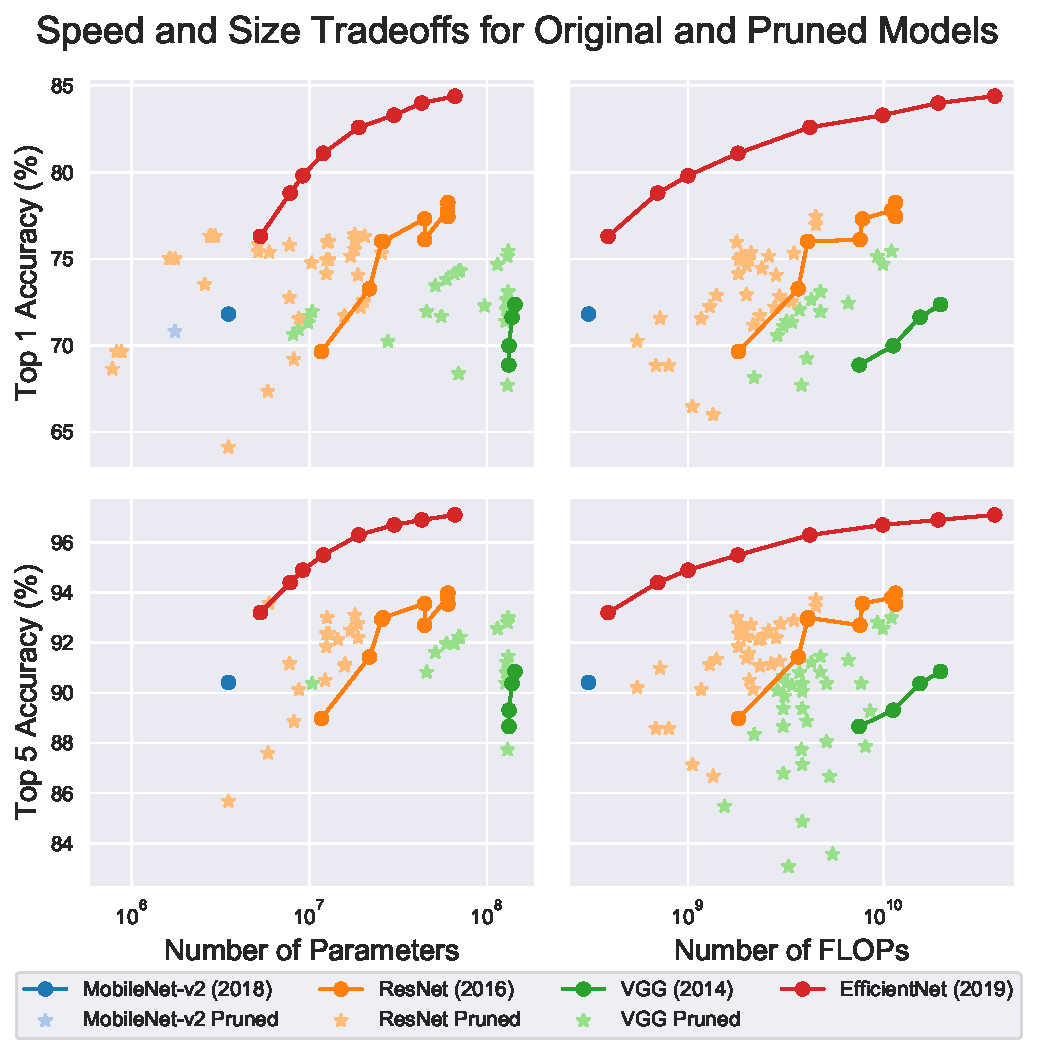
\includegraphics[width=\linewidth]{arch_vs_prune}
% \vspace{-3mm}
% \caption{Size and speed vs accuracy tradeoffs for different pruning methods and families of architectures. Pruned models sometimes outperform the original architecture, but rarely outperform a better architecture.}
% \label{fig:arch_vs_prune}
% \end{center}
% \end{figure}

% % ------------------------------------------------
% \subsection{Lottery Ticket Hypothesis}
% % ------------------------------------------------

% There has been a recent explosion of interest in the \textit{Lottery Ticket Hypothesis} \cite{lottery-ticket}. Informally, this hypothesis states that there are sparse subnetworks within a given model that 1) can be trained to equal or exceed the performance of the original model, and 2) depend on the initialization of the model, rather than merely the set of nonzeros chosen.
% The intuition behind the name is that these subnetworks have ``won the lottery'' with respect to initialization. Claim (1) follows from the general efficacy of pruning methods. Consequently, the investigation of the lottery ticket hypothesis centers on whether claim (2) holds; this is typically formulated as the question of whether retraining from scratch outperforms retraining from the pruned network's initial parameter values.
% % i.e., whether one must take into account the initialization when identifying the subnetwork, or whether it is only the pattern of nonzeros that matters.
% % As discussed above, the presence of a sparse subnetwork that outperforms the dense network has been demonstrated by numerous pruning papers.
% This question is interesting for at least two reasons:
% \begin{enumerate}
%     \itemsep2pt
%     \vspace{-3mm}
%     \item If the initialization from a fully-trained model significantly outperforms a random initialization, then obtaining peak efficiency requires a time consuming process of training and pruning. In contrast, if random initializations are just as good, one might be able to design or learn patterns of sparsity before running any training at all. \citet{snip} have already demonstrated that this is possible to some extent, though it does not yet appear to achieve the same performance as methods that use trained models \cite{lottery-ticket-followup}.
%     % \item If it is only the pattern of nonzeros that matters, it would likely be easier to design or learn patterns of nonzeros \textit{a priori} and obtain efficient, sparse models before running any training at all. [snip] has already demonstrated that this is possible to some extent, though it does not yet appear to achieve the same performance as methods that use the initialization or final trained model [lottery-ticket-followup].
%     \item The lottery ticket hypothesis is a bet against non-convex optimizers, in the sense that it holds only if the quality of the final solution depends on the initial parameter values. % To see this, consider that retraining from scratch should never perform worse that retraining from the initial parameter values given a sufficiently good optimizer, since the optimizer could, at the very least, begin
%     %1) if the lottery ticket hypothesis holds, a pruned network reset to its ``true'' initialization will outperform the same network reinitialized randomly; and 2) an oracle optimizer would obtain an equally good network regardless of the initialization. Therefore, we should expect the lottery ticket hypothesis to hold only if the optimizer used finds solutions of different quality depending on the initialization.
%     \vspace{-6mm}
% \end{enumerate}
% Multiple papers have confirmed the lottery ticket hypothesis for ResNet-50 on ImageNet \cite{google-state-of-sparsity, rethinking-net-pruning, stabilizing-lottery-tix}, and there is evidence that it holds for Transformer networks on language tasks \cite{google-state-of-sparsity} and other image classification networks on ImageNet \cite{lottery-transfer, lottery-ticket-followup}. However, the lottery ticket hypothesis does not always appear to hold. \citet{rethinking-net-pruning} show that retraining a pruned model from scratch can outperform the pruned model, and consistently does so  when allowing pruned models to train for longer than the original (so that the total number of \texttt{parameters} $\times$ \texttt{updates} remains close to constant). In light of this, recent work by Frankle \cite{lottery-ticket-followup, stabilizing-lottery-tix} (reproduced by \citet{lottery-transfer}) has shown that a simple modification of the lottery ticket hypothesis does always seem to hold. Namely, if instead of retraining from the initial parameter values, one retrains from the parameter values early in training (e.g., after one epoch), one consistently obtains a final model that outperforms those obtained by retraining from scratch. \citet{lottery-ticket-followup} also demonstrate that selecting which parameters to keep later in training tends to work better than doing so earlier.%, though selecting them only a few epochs into training can still yield a good pruned model.

% An interesting extension of the lottery ticket hypothesis is that of \cite{lottery-transfer}, who demonstrate that the sparse subnetworks in question can generalize across datasets and optimizers. In more detail, they show that if one prunes a neural network trained on one dataset, resets the non-pruned network parameters to their values early in training, and then trains this initial model on a new dataset (or with a new optimizer), the result is consistently better than randomly initializing the same network on the new dataset. Unsurprisingly, they find that initial models derived from larger datasets tend to yield better final accuracies than those from smaller datasets. More surprisingly, they find that initial models from \textit{large} datasets generalize better than initial models from the \textit{same} dataset when the latter dataset is small.

% % ------------------------------------------------
% \subsection{Other Findings}
% % ------------------------------------------------

% One consistent finding is that sparse models tend to outperform dense ones for a given number of parameters. \citet{snip-followup} show that increasing the nominal size of ResNet-20 on CIFAR-10 while sparsifying to hold the number of parameters constant decreases the error rate. \citet{wavernn} obtain a similar result for audio synthesis, as do \citet{openai-block-sparse} for a variety of additional tasks across various domains. Perhaps most compelling of all are the many results, including in Figure~\ref{fig:arch_vs_prune}, showing that pruned models can obtain higher accuracies than the original models from which they are derived. This demonstrates that sparse models can not only outperform dense counterparts with the same number of parameters, but sometimes dense models with even more parameters. % assuming one could add parameters to these models without harming their accuracies, these pruned models would also be instances of sparse models outperforming dense ones with the same number of parameters.

% There are also various credible findings in papers specifically attempting to improve the community's understanding of pruning in general.
% \citet{han-sparse-how} demonstrate that, for various models on large-scale image classification tasks, more granular sparsity consistently yields better accuracy for a given fraction of nonzeros. However, when measuring size by actual memory consumption instead of number of nonzeros, coarser sparsity can be better. This is because the latter reduces the overhead from storing nonzero indices by sharing one index between multiple nonzeros and sometimes reducing the necessary bit depth for indices.

% A more perplexing finding is that of \cite{prune-largest}. At least on CIFAR-10, they find that pruning the \textit{largest}-magnitude weights performs better than pruning the \textit{smallest}-magnitude weights, as long as the network is large enough to avoid underfitting. They show that this relates to the amount of ``instability'' introduced into the network, as measured by drop in validation accuracy immediately after pruning. This finding is surprising since pruning papers often frame their goal in terms of preserving the model's initial behavior. It is not yet clear how to reconcile this finding with the somewhat contrary result that current methods consistently perform better than random pruning (which one would expect to cause more instability).


%================================================================
\section{Missing Controlled Comparisons}
%================================================================

%!TEX root = doc.tex
%!TEX output_directory = aux

While there do appear to be a few general and consistent findings in the pruning literature (see the previous section), by far the clearest takeaway is that pruning papers rarely make direct and controlled comparisons to existing methods. This lack of comparisons stems largely from a lack of experimental standardization and the resulting fragmentation in reported results. This fragmentation makes it difficult for even the most committed authors to compare to more than a few existing methods.
% Section~\ref{sec:lessons}
 % Moreover, when such comparisons are made, they often fail to account

% literature suffers from a dearth of meaningful comparisons between methods. This deficiency stems from a lack of experimental standardization, which makes it impractical for new authors to compare to more than a small number of existing methods. % Below, we provide evidence for these claims and highlight pitfalls that should be avoided for future comparisons. % However, as we will discuss in the next section, this is not a result of individual authors making poor choices, but of the field as a whole failing to converge on standard experimental setups.
% In this section, we argue that such a lack of comparisons exists, and that this lack presents a barrier to progress within this field.

% ------------------------------------------------
% \vspace{-1.5mm}
\subsection{Omission of Comparison}
% \vspace{-.25mm}
% ------------------------------------------------

Many papers claim to advance the state of the art, but don't compare to other methods---including many published ones---that make the same claim. % This implies that many such claims are not adequately justified.

% Dozens of papers in our corpus purport to introduce a method that surpasses the current state-of-the-art. A necessary condition for this claim to be true is that the paper outperform any other nominally ``state-of-the-art'' methods existing at the time the paper is written. However, few if any papers in the past decade have been able to demonstrate that they do this. % Indeed, they have not even \textit{compared} to many papers that have a claim to be state-of-the-art.

% ------------------------
% \subsubsection{Ignoring Pre-2010s Methods}
\vspace{-2mm}
\paragraph{Ignoring Pre-2010s Methods}
% ------------------------

% To see this, consider first the fact that t
There was already a rich body of work on neural network pruning by the mid 1990s (see, e.g., Reed's survey \cite{reed_pruning_1993}), which has been almost completely ignored except for Lecun's Optimal Brain Damage \cite{optimal-brain-damage} and Hassibi's Optimal Brain Surgeon \cite{optimal-brain-surgeon}. Indeed, multiple authors have rediscovered existing methods or aspects thereof, with \citet{learning-both} reintroducing the magnitude-based pruning of \citet{janowsky_pruning_1989}, \citet{snip} reintroducing the saliency heuristic of \citet{mozer_skeletonization:_1989}, and \citet{soft-filter-pruning} reintroducing the practice of ``reviving'' previously pruned weights described in \citet{early-brain-damage}.
\begin{figure}[t]
\begin{center}
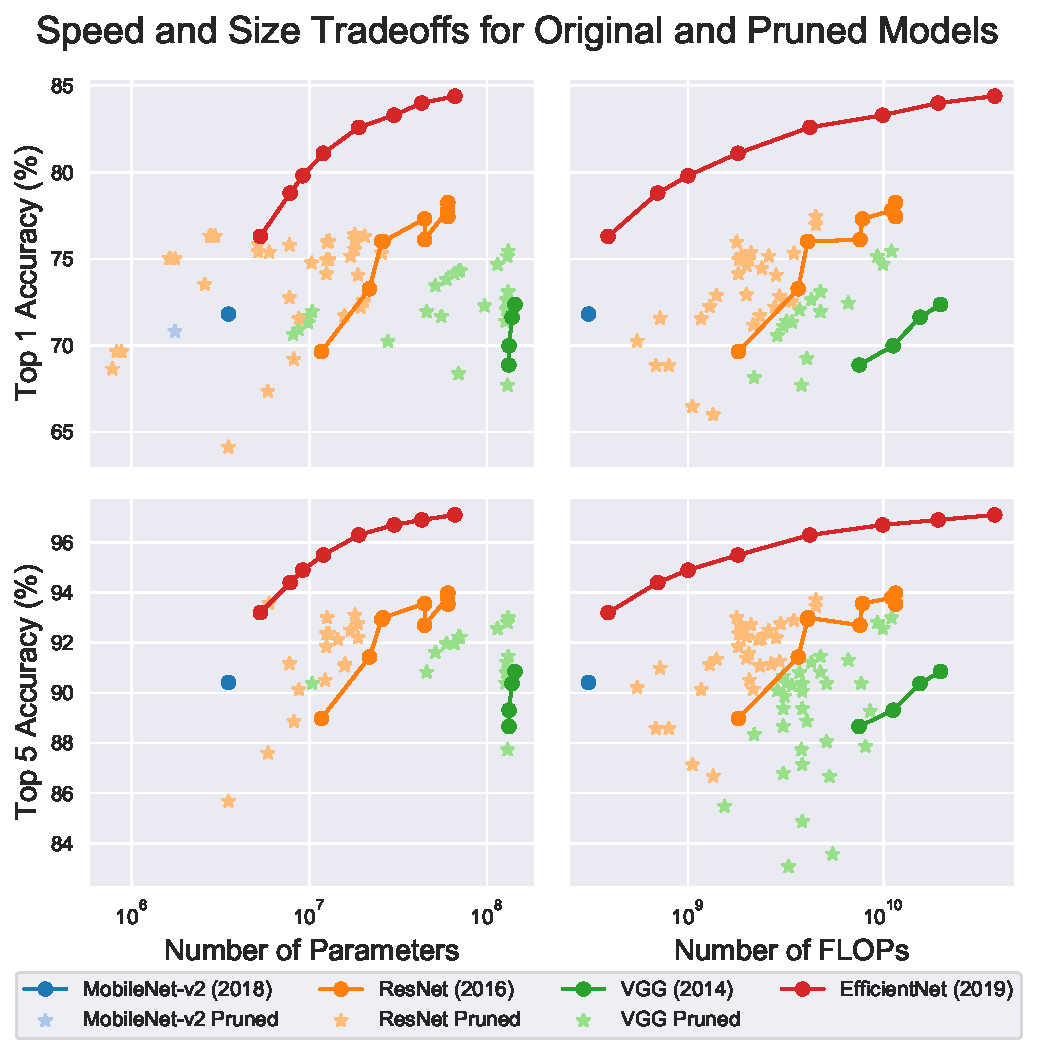
\includegraphics[width=\linewidth]{arch_vs_prune}
\vspace{-3mm}
\caption{Size and speed vs accuracy tradeoffs for different pruning methods and families of architectures. Pruned models sometimes outperform the original architecture, but rarely outperform a better architecture.}
\label{fig:arch_vs_prune}
\end{center}
\end{figure}
\vspace{3mm}

% ------------------------
% \subsubsection{Ignoring Recent Methods}
% \vspace{-3em}
\paragraph{Ignoring Recent Methods}
% ------------------------

% Even under the strong assumption that all pre-2010 methods are inferior, t
Even when considering only post-2010 approaches, there are still virtually no methods that have been shown to outperform all existing ``state-of-the-art'' methods. This follows from the fact, depicted in the top plot of Figure~\ref{fig:paper_comparisons_hist}, that there are dozens of modern papers---including many affirmed through peer review---that have never been compared to by any later study.
% We define a comparison here as reporting any numeric result for one's own method alongside any numeric result for the same (dataset, model) pair from the method in question. As we will discuss later in the section, this is a lax standard that does not necessarily imply that one method has meaningfully outperformed the other.
% Any of the associated authors could claim to have the best pruning method, since no one has ever even attempted to demonstrate otherwise.
% As emphasized previously, we believe that the main reason for this lack of comparison is not sloppiness or ill intent, but the reality that comparing to any given method is difficult or even impossible.

A related problem is that papers tend to compare to few existing methods. In the lower plot of Figure~\ref{fig:paper_comparisons_hist}, we see that more than a fourth of our corpus does not compare to any previously proposed pruning method, and another fourth compares to only one. Nearly all papers compare to three or fewer. This might be adequate if there were a clear progression of methods with one or two ``best'' methods at any given time, but this is not the case. % These observations hold for both published and unpublished papers.
% An additional and enabling factor appears to be lax community standards. In the lower plot of Figure~\ref{fig:paper_comparisons_hist}, we see that more than a fourth of our corpus \textit{does not compare to any existing pruning method}, and another fourth compares to only one. Nearly all papers compare to three or fewer. This might be adequate if there were a clear progression of methods with one or two ``best'' methods at any given time, but as this section argues, this is not the case. These facts hold for both published and unpublished papers.

% Even among modern papers, however, there are dozens of papers that can claim to be state-of-the-art, as measured by the absence

% Unfortunately, even if there were no methodological issues whatsoever with any of their experimental comparisons, this usually cannot have been the case even at the time the papers were written.

% In Figure~\ref{fig:paper_comparisons_hist}, we plot histograms of the number of papers comparing to a given method (top) and number of other papers that a given new paper compares to (bottom). The far left bar on the upper plot shows that there are over 30 papers that \textit{have never been compared to by anyone}, at least among all the papers we were able to find. In other words, there are at least 30 papers that can claim to be ``state-of-the-art''.

% In the lower plot, we see that the review standards for being ``state-of-the-art'' are remarkably lax.

\begin{figure}[h]
\begin{center}
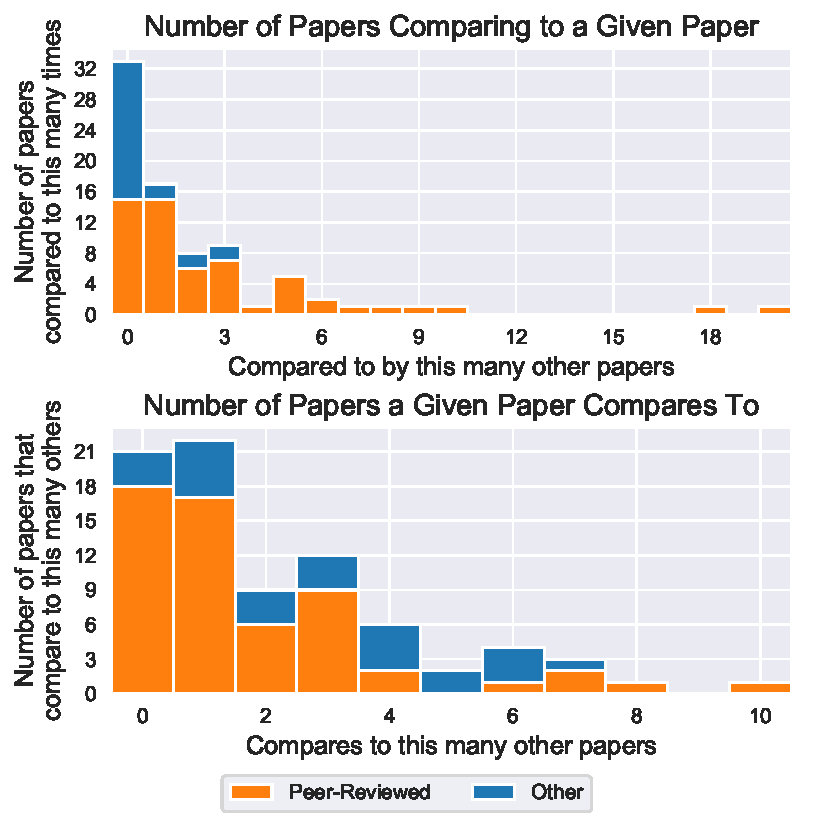
\includegraphics[width=\linewidth]{paper_comparisons_hist}
\caption{Reported comparisons between papers.
% \textit{Top)} More than a third of the papers in our corpus have no other paper purporting to outperform them. \textit{Bottom)} Most papers compare to at most one other paper, and often none. Peer-reviewed papers are less likely to be ignored, but do not make more comparisons to existing methods. % These patterns hold regardless of whether a paper is peer-reviewed.}
}
\label{fig:paper_comparisons_hist}
\end{center}
\end{figure}

% ------------------------------------------------
\subsection{Dataset and Architecture Fragmentation}
% ------------------------------------------------

% It appears that a major underlying cause for the absence of meaningful comparisons is the lack of standard datasets, architectures, and metrics. % This means that comparing to a given existing paper usually necessitates additional code to match the experimental setting of the particular paper in question, assuming the setting is reproducible enough to be matched at all. A few exemplary authors work hard to match many earlier experiments (e.g., \cite{dai-info-bottleneck, rethinking-net-pruning}), but, understandably, most avoid this as much as possible. % This causes new papers to introduce new experimental setups, creating a vicious cycle.
% This results in a self-perpetuating cycle of
% In this section, we describe the extent of the fragmentation in datasets and architectures. % We believe that this extreme fragmentation suggests a desparate need for standard benchmarks. % and by implication the desparate need for some form of standardization.

% The second core problem, which contributes to the first, is that there is no standard set of datasets and models that everyone uses. This
% results in 1) most comparisons involving at most one or two (dataset, architecture) combinations, 2) no ability to compare to other papers ``for free''---

% . This is far too little to establish that one method is superior to another, except perhaps in the case of perfectly representative tasks and large, consistent differences.

% As a first indication of how fragmented the reported results are, consider that

Among \npapers papers, we found results using 49 datasets, 132 architectures, and 195 (dataset, architecture) combinations. As shown in Table~\ref{tbl:common_combos}, even the most common combination of dataset and architecture---VGG-16 on ImageNet\footnote{We adopt the common practice of referring to the ILSVRC2012 training and validation sets as ``ImageNet.''} \cite{imagenet}---is used in only 22 out of \npapers papers. Moreover, three of the top six most common combinations involve MNIST \cite{mnist}. As \citet{google-state-of-sparsity} and others have argued, using larger datasets and models is essential when assessing how well a method works for real-world networks. MNIST results may be particularly unlikely to generalize, since this dataset differs significantly from other popular datasets for image classification. In particular, its images are grayscale, composed mostly of zeros, and possible to classify with over 99\% accuracy using simple models \cite{mnist-page}.

% since this dataset has several unusual properties. First, unlike other popular datasets for vision classification tasks, MNIST is not composed of natural images, but instead grayscale images that are mostly zeros. Second, the variance of image patterns across samples is smaller than other natural image datasets. Finally, even simple classifiers can obtain over 99\% test accuracy \cite{mnist-page} on MNIST.

% These properties mean that methods that work on MNIST may not work on larger-scale problems.

% TODO maybe switch to (dataset, model, efficiency metric, quality metric) ?

% \begin{table}[h!]
% \begin{centering}
% \begin{tabular}{ll|c}
% \multicolumn{2}{c}{(Dataset, Architecture) Pair} & \shortstack{Number of Papers \\ using Pair} \\
% % \vspace*{2pt}
% \toprule
% ImageNet & VGG-16 & 22 \\
% ImageNet & ResNet-50 & 15 \\
% MNIST & LeNet-5-Caffe & 14 \\
% CIFAR-10 & ResNet-56 & 14 \\
% MNIST & LeNet-300-100 & 12 \\
% MNIST & LeNet-5 & 11 \\
% ImageNet & CaffeNet & 10 \\
% CIFAR-10 & CIFAR-VGG (Torch) & 8 \\
% ImageNet & AlexNet & 8 \\
% ImageNet & ResNet-18 & 6 \\
% ImageNet & ResNet-34 & 6 \\
% CIFAR-10 & ResNet-110 & 5 \\
% CIFAR-10 & PreResNet-164 & 4 \\
% CIFAR-10 & ResNet-32 & 4 \\
% % \bottomrule
% % ImageNet, ResNet-101 & 3 \\
% % ImageNet, GoogLeNet & 3 \\
% % CIFAR-100, PreResNet-164 & 3 \\
% % CIFAR-10, VGG-19 & 3 \\
% % CIFAR-10, ResNet-20 & 3 \\
% % CIFAR-10, VGG-netslim & 3 \\
% % CIFAR-10, ResNet-18 & 3 \\
% % CUB200-2011, VGG-16 & 3 \\
% % CIFAR-100, VGG-Torch-CIFAR10 & 3 \\
% % CIFAR-10, DenseNet-40 & 3 \\
% % CIFAR-100, VGG-19 & 2 \\
% % CIFAR-10, Cifar-net & 2 \\
% % CamVid, SegNet & 2 \\
% % CIFAR-10, WRN-28-10 & 2 \\
% % CIFAR-10, WRN-22-8 & 2 \\
% % CIFAR-100, DenseNet-40 & 2 \\
% % ImageNet, VGG-Tiny & 2 \\
% % ImageNet, VGG-GAP & 2 \\
% % ImageNet, VGG-A+BN-noDrop & 2 \\
% % MNIST, fc300-1000-300 & 2 \\
% % MNIST, fc500-300-100 & 2 \\
% % ImageNet, SqueezeNet & 2 \\
% % CIFAR-10, PreResNet-110 & 2 \\
% % CIFAR-100, WRN-28-10 & 2 \\
% % ImageNet, MobileNet & 2 \\
% % Pascal VOC 2007, VGG-16 & 2 \\
% % CIFAR-10, Plain-20 & 2 \\
% % CIFAR-100, WRN-16-4 & 2 \\
% % CIFAR-10, ResNet-50 & 2 \\
% \end{tabular}
% \end{centering}
% \caption{All combinations of dataset and architecture used in at least 4 out of \npapers papers.
% % To have a clear state-of-the-art, there should be numerous combinations used by a large fraction of papers.
% }
% \label{tbl:common_combos}
% \vspace*{1mm}
% \end{table}

% ------------------------------------------------
\subsection{Metrics Fragmentation}
% ------------------------------------------------

\begin{table}[t]
\begin{centering}
\begin{tabular}{ll|c}
\multicolumn{2}{c}{(Dataset, Architecture) Pair} & \shortstack{Number of Papers \\ using Pair} \\
% \vspace*{2pt}
\toprule
ImageNet & VGG-16 & 22 \\
ImageNet & ResNet-50 & 15 \\
MNIST & LeNet-5-Caffe & 14 \\
CIFAR-10 & ResNet-56 & 14 \\
MNIST & LeNet-300-100 & 12 \\
MNIST & LeNet-5 & 11 \\
ImageNet & CaffeNet & 10 \\
CIFAR-10 & CIFAR-VGG (Torch) & 8 \\
ImageNet & AlexNet & 8 \\
ImageNet & ResNet-18 & 6 \\
ImageNet & ResNet-34 & 6 \\
CIFAR-10 & ResNet-110 & 5 \\
CIFAR-10 & PreResNet-164 & 4 \\
CIFAR-10 & ResNet-32 & 4 \\
% \bottomrule
% ImageNet, ResNet-101 & 3 \\
% ImageNet, GoogLeNet & 3 \\
% CIFAR-100, PreResNet-164 & 3 \\
% CIFAR-10, VGG-19 & 3 \\
% CIFAR-10, ResNet-20 & 3 \\
% CIFAR-10, VGG-netslim & 3 \\
% CIFAR-10, ResNet-18 & 3 \\
% CUB200-2011, VGG-16 & 3 \\
% CIFAR-100, VGG-Torch-CIFAR10 & 3 \\
% CIFAR-10, DenseNet-40 & 3 \\
% CIFAR-100, VGG-19 & 2 \\
% CIFAR-10, Cifar-net & 2 \\
% CamVid, SegNet & 2 \\
% CIFAR-10, WRN-28-10 & 2 \\
% CIFAR-10, WRN-22-8 & 2 \\
% CIFAR-100, DenseNet-40 & 2 \\
% ImageNet, VGG-Tiny & 2 \\
% ImageNet, VGG-GAP & 2 \\
% ImageNet, VGG-A+BN-noDrop & 2 \\
% MNIST, fc300-1000-300 & 2 \\
% MNIST, fc500-300-100 & 2 \\
% ImageNet, SqueezeNet & 2 \\
% CIFAR-10, PreResNet-110 & 2 \\
% CIFAR-100, WRN-28-10 & 2 \\
% ImageNet, MobileNet & 2 \\
% Pascal VOC 2007, VGG-16 & 2 \\
% CIFAR-10, Plain-20 & 2 \\
% CIFAR-100, WRN-16-4 & 2 \\
% CIFAR-10, ResNet-50 & 2 \\
\end{tabular}
\end{centering}
\caption{All combinations of dataset and architecture used in at least 4 out of \npapers papers.
% To have a clear state-of-the-art, there should be numerous combinations used by a large fraction of papers.
}
\label{tbl:common_combos}
\vspace*{1mm}
\end{table}

As depicted in Figure~\ref{fig:prune_grid}, papers report a wide variety of metrics and operating points, making it difficult to compare results. Each column in this figure is one (dataset, architecture) combination taken from the four most common combinations\footnote{We combined the results for AlexNet and CaffeNet, which is a slightly modified version of AlexNet \cite{caffenet}, since many authors refer to the latter as ``AlexNet,'' and it is often unclear which model was used.}, excluding results on MNIST. Each row is one pair of metrics. Each curve is the efficiency vs accuracy tradeoff obtained by one method.\footnote{Since what counts as one method can be unclear, we consider all results from one paper to be one method except when two or more named methods within the paper report using at least one identical x-coordinate (i.e., when the paper's results can't be plotted as one curve).} Methods are color-coded by year.

It is hard to identify any consistent trends in these plots, aside from the existence of a tradeoff between efficiency and accuracy. A given method is only present in a small subset of plots. Methods from later years do not consistently outperform methods from earlier years. Methods within a plot are often incomparable because they report results at different points on the x-axis. Even when methods are nearby on the x-axis, it is not clear whether one meaningfully outperforms another since neither reports a standard deviation or other measure of central tendency. Finally, most papers in our corpus do not report any results with any of these common configurations.

\begin{figure*}[hbt!]
\begin{center}
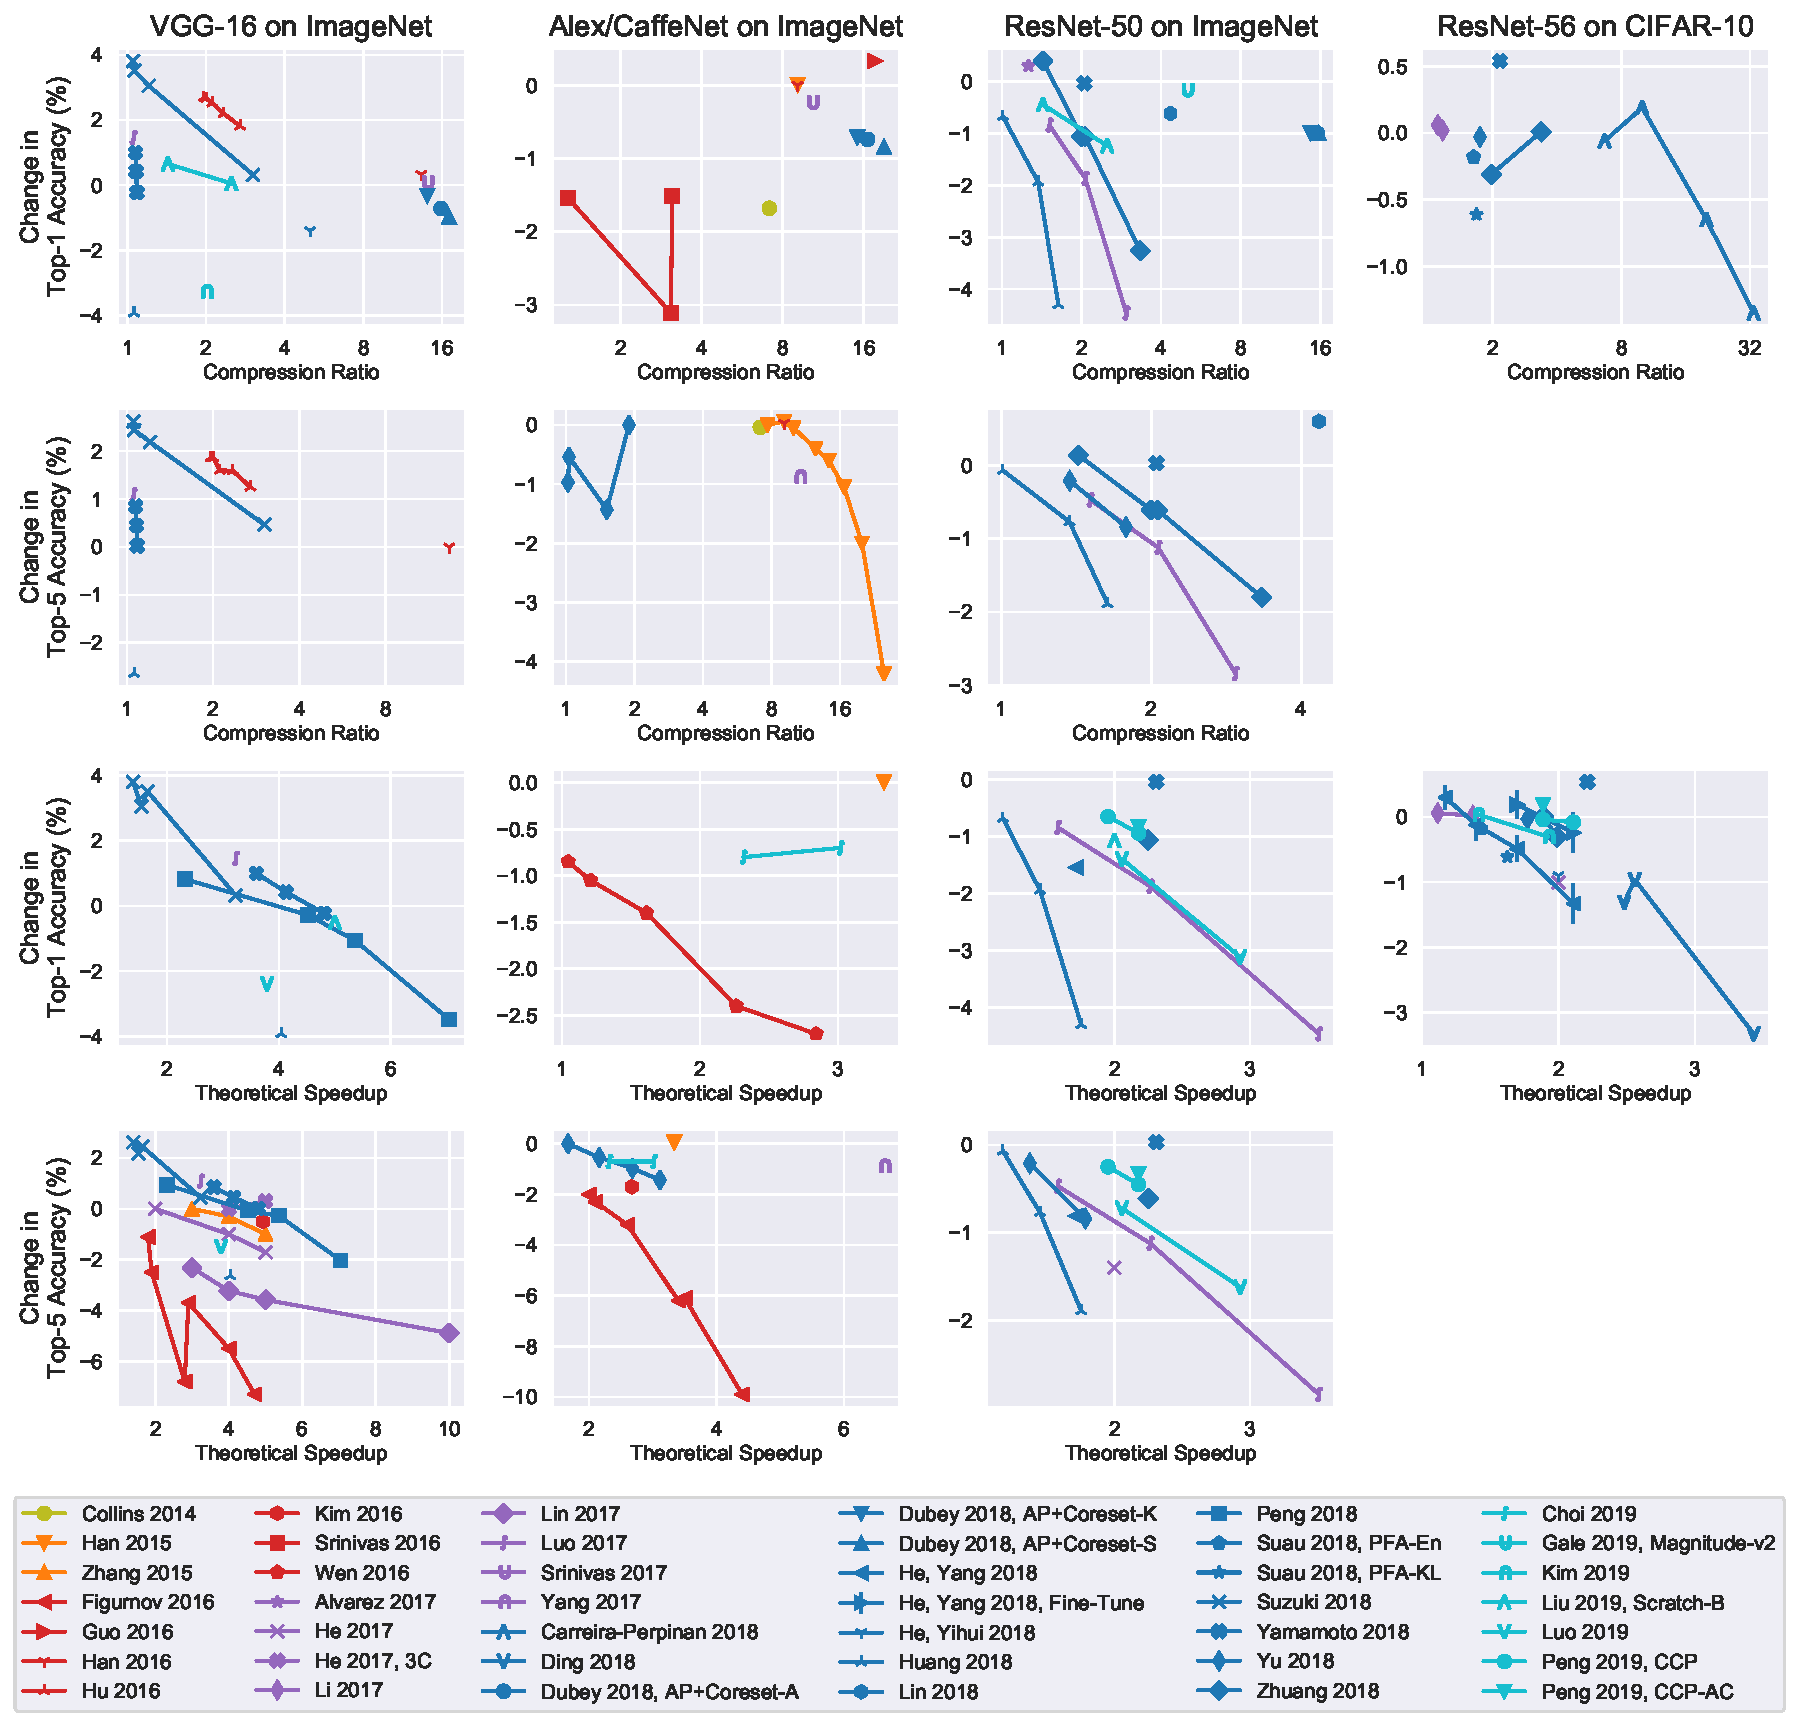
\includegraphics[width=\linewidth]{all_pruning_curves}
\caption{Fragmentation of results. Shown are all self-reported results on the most common (dataset, architecture) combinations. Each column is one combination, each row shares an accuracy metric (y-axis), and pairs of rows share a compression metric (x-axis). Up and to the right is always better. Standard deviations are shown for He 2018 on CIFAR-10, which is the only result that provides any measure of central tendency.
% Observe that each combination of dataset, architecture, and metrics (one subplot) has results from only a small fraction of the papers. Even when these factors agree, different papers often obtain incomparable results since they are better in one respect but worse in another. Methods are color-coded by year, and there appears to be no clear progress over time. Later methods are sometimes strictly worse than earlier ones.
As suggested by the legend, only 37 out of the \npapers papers in our corpus report any results using any of these configurations.}
\label{fig:prune_grid}
\end{center}
\vspace{-4mm}
\end{figure*}

% ------------------------------------------------
% \subsection{Incomplete Characterization of Results}
\subsection{Incomplete Characterization of Results}
% ------------------------------------------------

% As shown in Figure~\ref{fig:prune_grid}, many methods are not comparable because they use different combinations of models, datasets, and metrics, as well as disparate efficiency levels in their efficiency vs accuracy tradeoff curves.
% Recall that a pruning method must balance both efficiency and accuracy, and that this tradeoff can be characterized in terms of a curve of (efficiency, accuracy) pairs associated with a given dataset and model. As we discussed previously, methods with non-overlapping ranges of their reported curves, or with different datasets and models, cannot be directly compared.

If all papers reported a wide range of points in their tradeoff curves across a large set of models and datasets, there might be some number of direct comparisons possible between any given pair of methods. %, even if the overall sets of reported results differed.
% One factor exacerbating this is that authors report few (dataset, architecture) pairs as well as few measurements to characterize each pair's tradeoff curve.
As we see in the upper half of Figure~\ref{fig:numresults_stats}, however, most papers use at most three (dataset, architecture) pairs; and as we see in the lower half, they use at most three---and often just one---point to characterize each curve. Combined with the fragmentation in experimental choices, this means that different methods' results are rarely directly comparable. Note that the lower half restricts results to the four most common (dataset, architecture) pairs.

\begin{figure}[h]
\begin{center}
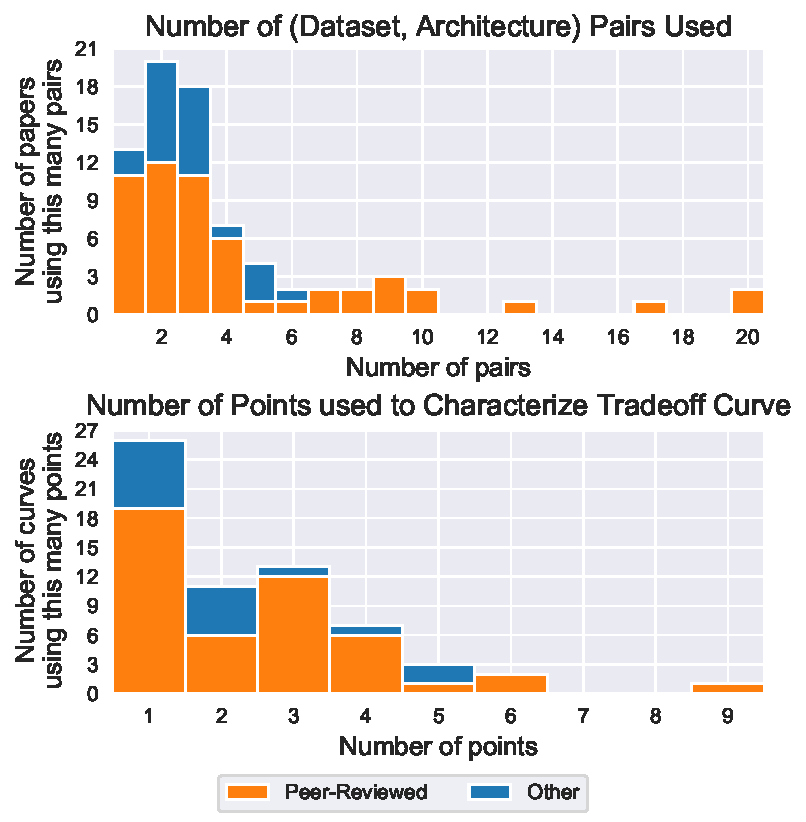
\includegraphics[width=\linewidth]{numresults_stats}
\caption{Number of results reported by each paper, excluding MNIST. \textit{Top)} Most papers report on three or fewer (dataset, architecture) pairs. \textit{Bottom)} For each pair used, most papers characterize their tradeoff between amount of pruning and accuracy using a single point in the efficiency vs accuracy curve. In both plots, the pattern holds even for peer-reviewed papers.}
\label{fig:numresults_stats}
\end{center}
\end{figure}

% ------------------------------------------------
\subsection{Confounding Variables} \label{sec:confounding}
% ------------------------------------------------
% Suppose that Paper A compares to Paper B using a large number of the same architectures on the same datasets, reports the same metrics, evaluates their method at numerous operating points, which are themselves identical to those used in Paper B, and obtains better results than those reported in Paper B at all operating points. Can we conclude that Paper A's method outperforms Paper B's?
% Unfortunately, we may not be able to. The problem is that using reported results fails to account for numerous confounding variables. Some variables of particular interest include:

% % ------------------------
% \subsubsection{Common Confounders}
% % ------------------------
Even when comparisons include the same datasets, models, metrics, and operating points, other confounding variables still make meaningful comparisons difficult. Some variables of particular interest include:
\begin{itemize}[leftmargin=4mm]
    % \itemsep-1.5pt
    \itemsep2pt
    \vspace{-3.5mm}
    % \item Initial trained parameters. Initially worse models might be easier or harder to improve.
    \item Accuracy and efficiency of the initial model
    \item Data augmentation and preprocessing
    \item Random variations in initialization, training, and fine-tuning. This includes choice of optimizer, hyperparameters, and learning rate schedule.
    \item Pruning and fine-tuning schedule
    % (how often to prune throughout fine-tuning, how much pruning at a time, total fine-tuning epochs, etc).
    % \item Fine-tuning settings, such as number of epochs of fine-tuning.
    \item Deep learning library. Different libraries are known to yield different accuracies for the same architecture and dataset \cite{unreproducibleCurtis, unreproducible3} and may have subtly different behaviors \cite{kerasBnWeird}.
    \item Subtle differences in code and environment that may not be easily attributable to any of the above variations \cite{unreproducible0, unreproducible1, unreproducible4}.
\end{itemize}
% \vspace{-10pt}

In general, it is not clear that any paper can succeed in accounting for all of these confounders unless that paper has both used the same code as the methods to which it compares and reports enough measurements to average out random variations. This is exceptionally rare, with \citet{google-state-of-sparsity} and \citet{rethinking-net-pruning} being arguably the only examples. Moreover, neither of these papers introduce novel pruning methods \textit{per se} but are instead inquiries into the efficacy of existing methods.

% ------------------------
% \subsubsection{Common Mitigation Practices can be Inadequate}
% \paragraph{Common Mitigation Practices can be Inadequate}
% ------------------------

Many papers attempt to account for subsets of these confounding variables. A near universal practice in this regard is reporting change in accuracy relative to the original model, in addition to or instead of raw accuracy. This helps to control for the accuracy of the initial model. However, as we demonstrate in Section~\ref{sec:bench}, this is not sufficient to remove initial model as a confounder. Certain initial models can be pruned more or less efficiently, in terms of the accuracy vs compression tradeoff. This holds true even with identical pruning methods and all other variables held constant.

% we did not find any empirical or theoretical evidence that examining only changes is sufficient to remove initial model accuracy as a confounder. I.e., it could be the case that initially worse models are easier (or harder) to prune without accuracy degradation.

%The thinking is that a method that reduces accuracy from 92\% to 91\% should be considered worse than a method that increases it from 88\% to 90\%, even though the latter obtains a lower final accuracy. This is probably correct, but we did not find any empirical or theoretical evidence that examining only changes is sufficient to remove initial model accuracy as a confounder. I.e., it could be the case that initially worse models are easier (or harder) to prune without accuracy degradation.
% It could be the case that a worse model is likely easier to ``improve'' by pruning, if only because fine-tuning affords one a chance to get less unlucky than whomever initially trained the model (and possibly to apply more recent training methods).

% ------------------------
% \subsubsection{Impact of Fine-Tuning}
% \subsubsection{Impact of Confounders}
% \paragraph{Impact of Confounders}
% ------------------------

% One might wonder whether the impact of these confounders is actually significant relative to that of pruning method choice. % After all, random variations typically perturb accuracies for a given pruned model on ImageNet by less than half a percentage point [], and the relative efficacy of ImageNet image classifiers appears to hold even for novel large-scale datasets [].
\vspace{2mm}
There are at least two more empirical reasons to believe that confounding variables can have a significant impact. First, as one can observe in Figure~\ref{fig:prune_grid}, methods often introduce changes in accuracy of much less than 1\% at reported operating points. This means that, even if confounders have only a tiny impact on accuracy, they can still have a large impact on which method appears better. % This is particularly true in the absence of any sort of error bars.

\vspace{2mm}
Second, as shown in Figure~\ref{fig:magnitude_vs_nonmagnitude}, existing results demonstrate that different training and fine-tuning settings can yield nearly as much variability as different methods. Specifically, consider 1) the variability introduced by different fine-tuning methods for unstructured magnitude-based pruning (Figure 6 top) and 2) the variability introduced by entirely different pruning methods (Figure 6 bottom). The variability between fine-tuning methods is nearly as large as the variability between pruning methods.
%Specifically, consider two sets of tradeoff curves: 1) those for a single method (iterative, unstructured, magnitude-based pruning) using different implementations and fine-tuning practices, and 2) those for all other methods. If method made far more difference than training and fine-tuning, then the former set of curves should exhibit far less variation than the latter. As Figure~\ref{fig:magnitude_vs_nonmagnitude} depicts however, this is not the case---the within-method variation is nearly as large as the between-method variation.
 % As we see in , these two sets of curves appear to vary in quality as much as the tradeoff curves for different methods.
\begin{figure}[h]
\begin{center}
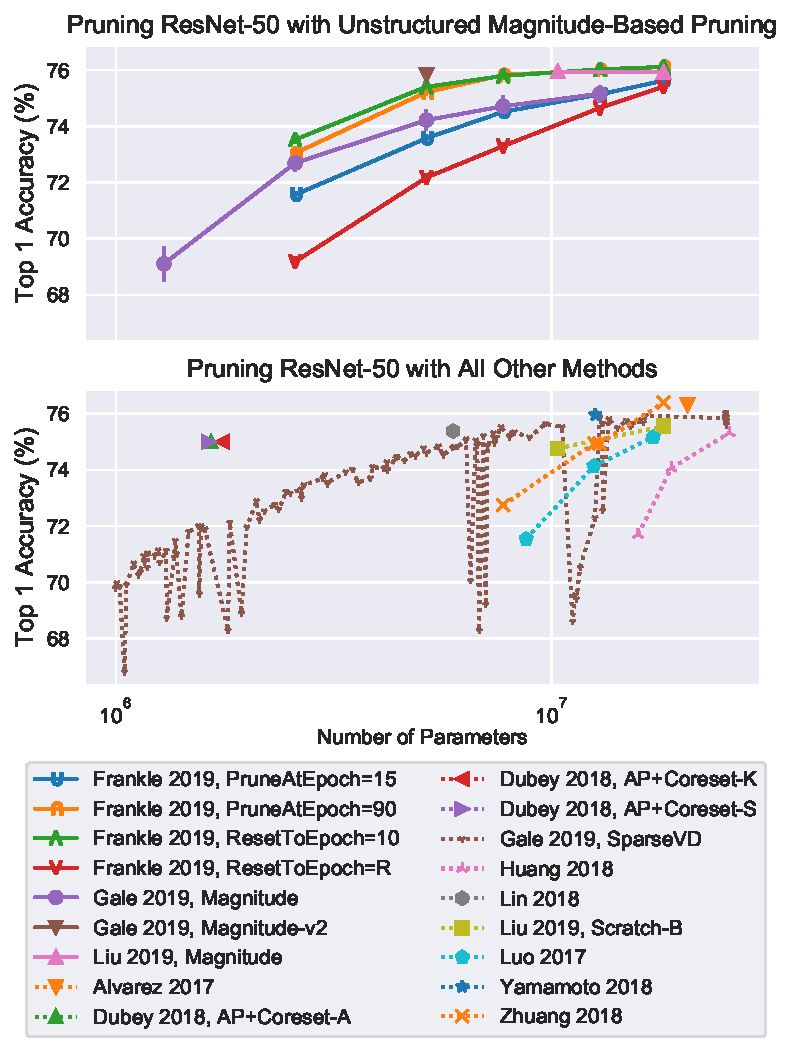
\includegraphics[width=\linewidth]{magnitude_vs_nonmagnitude}
\caption{Pruning ResNet-50 on ImageNet. Methods in the upper plot all prune weights with the smallest magnitudes, but differ in implementation, pruning schedule, and fine-tuning. The variation caused by these variables is similar to the variation across different pruning methods, whose results are shown in the lower plot. All results are taken from the original papers.}
\label{fig:magnitude_vs_nonmagnitude}
\end{center}
\vspace*{3mm}
\end{figure}


%================================================================
% \section{Why the Lack of Comparisons?}
% \vspace*{4mm}
\section{Further Barriers to Comparison}
%================================================================

%!TEX root = doc.tex
%!TEX output_directory = aux

% In the previous section, we provided evidence that the neural network pruning literature suffers from a severe lack of meaningful comparison between methods. In this section, we attempt to shed light on why this is. At a high level, our conclusion is that authors are behaving reasonably given the incentives with which they are presented and the difficulty of performing meaningful comparisons.

% In the previous section, we provided evidence that the neural network pruning literature suffers from a lack of apples-to-apples comparisons between methods. Might it be possible, however, to examine our aggregated results post-hoc and determine which methods are best? The answer appears to be no. In this section, we detail the barriers that we---and authors of pruning papers in general---encounter when attempting to compare existing methods.

% We have already discussed
% In the previous section, we discussed the fragmentation of datasets, models, metrics, and operating points, and how this fragmentation makes implementing controlled comparisons between methods difficult. Regrettably, these difficulties are largely inevitable so long as the literature remains fragmented.

% However, there are some ways in which the barriers to comparison can be lowered. In this section, we focus on preventable obstacles to comparison, which in most cases stem from the presentation and selection of results. In particular, papers often appear to not be written so as to facilitate future comparison to their proposed methods. We discuss several ways in which this manifests and how it increases the difficulty of meaningful comparison between methods. % In the next section, we will also discuss concrete practices to avoid these pitfalls.

In the previous section, we discussed the fragmentation of datasets, models, metrics, operating points, and experimental details, and how this fragmentation makes evaluating the efficacy of individual pruning methods difficult. In this section, we argue that there are additional barriers to comparing methods that stem from common practices in how methods and results are presented.% (or lack thereof) in the literature.

% In particular, papers often appear to not be written so as to facilitate future comparison to their proposed methods. We discuss several ways in which this manifests and how it increases the difficulty of meaningful comparison between methods.

 % a key factor is that many papers are not written with ``forwards compatiblity'' in mind. That is, they appear to not be written so as to facilitate future comparison to their proposed methods. In this section, we discuss several ways in which this manifests and how it increases the difficulty of meaningful comparison between methods.
% In addition to the fragmentation of datasets, models, metrics, and operating points already discussed, a key factor is that many papers are not written with ``forwards compatiblity'' in mind. That is, they appear to not be written so as to facilitate future comparison to their proposed methods. In this section, we discuss several ways in which this manifests and how it increases the difficulty of meaningful comparison between methods.

% % ------------------------------------------------
% \subsection{Practical Barriers}
% % ------------------------------------------------

% % As authors of papers on pruning are no doubt aware, f
% Fairly comparing one's own method to an existing method can require a great deal of work. At best, it requires reimplementing a pruning heuristic within one's own experimental infrastructure. At worst, it requires hooking into another author's source code to attempt---possibly without success---to exactly replicate their experimental conditions. And this is assuming that usable source code is even available. Because different papers use different models, datasets, and experimental setups, this high cost must be paid for each method to which one compares.

% Moreover, even if one has time to write all the needed code, one might still encounter computational limitations. As evidenced by the near total lack of error bars in Figure~\ref{fig:prune_grid}, training or fine-tuning large networks on large datasets is a slow and sometimes expensive process that few authors have the resources to carry out repeatedly. % are willing to carry out more than necessary.

% In short, we believe that authors fail to make many (rigorous) comparisons not for want of desire, but because doing so is extremely difficult. Combined with a review climate in which lackluster evaluations are adequate for even the best conferences, it is unsurprising that the literature has remained in its current state.

% % ------------------------------------------------
% \subsection{Lack of Forwards Compatibility}
% % ------------------------------------------------

% In addition to the practical barriers discussed above, many papers appear to not be written so as to facilitate future comparison to the presented method. In this section, we discuss several ways in which this manifests and how it increases the difficulty of meaningful comparison between methods. % Note that, in the spirit of collegiality, we will in some cases refrain from attributing omissions and mistakes to particular authors.

% % ------------------------------------------------
% % \subsection{Incomplete Characterization of Results}
% \subsection{Incomplete Characterization of Results}
% % ------------------------------------------------

% % As shown in Figure~\ref{fig:prune_grid}, many methods are not comparable because they use different combinations of models, datasets, and metrics, as well as disparate efficiency levels in their efficiency vs accuracy tradeoff curves.
% Recall that a pruning method must balance both efficiency and accuracy, and that this tradeoff can be characterized in terms of a curve of (efficiency, accuracy) pairs associated with a given dataset and model. As we discussed previously, methods with non-overlapping ranges of their reported curves, or with different datasets and models, cannot be directly compared.

% If all papers reported a wide range of points in their tradeoff curves across a large set of models and datasets, there might be some number of direct comparisons between any given pair of methods. %, even if the overall sets of reported results differed.
% % One factor exacerbating this is that authors report few (dataset, architecture) pairs as well as few measurements to characterize each pair's tradeoff curve.
% As we see in the upper half of Figure~\ref{fig:numresults_stats}, however, most papers use at most three (dataset, architecture) pairs; and as we see in the lower half, they use at most three---and often just one---point to characterize each curve. Combined with the fragmentation in experimental choices, this means that different methods' results rarely overlap. Note that the lower half restricts results to the four most common (dataset, architecture) pairs.

% \begin{figure}[h]
% \begin{center}
% 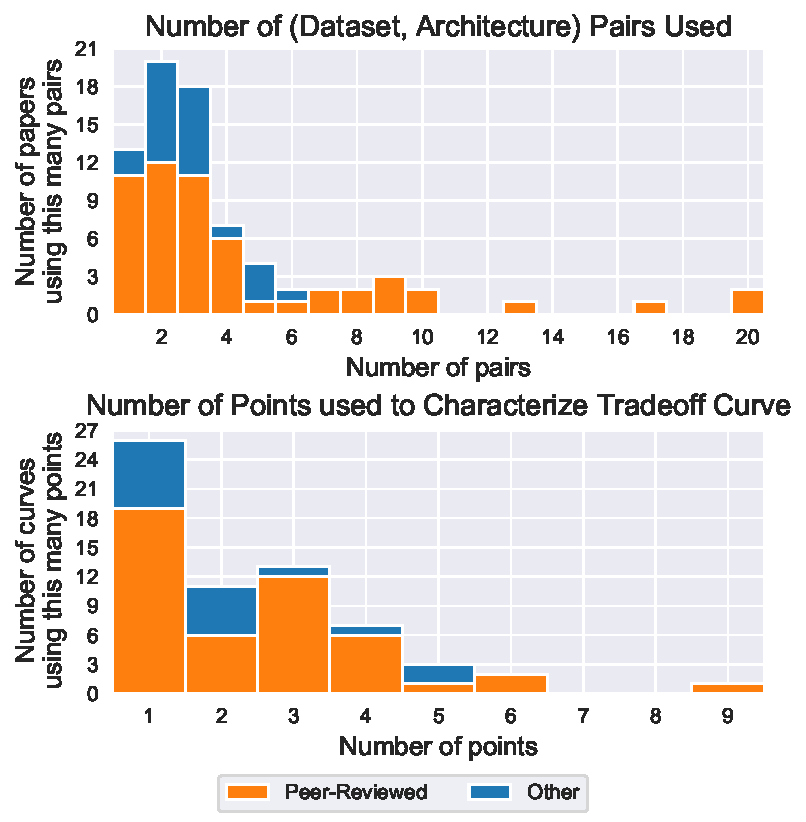
\includegraphics[width=\linewidth]{numresults_stats}
% \caption{Number of results reported by each paper, excluding MNIST. \textit{Top)} Most papers report on three or fewer (dataset, architecture) pairs. \textit{Bottom)} For each pair used, most papers characterize their tradeoff between amount of pruning and accuracy using a single point in the efficiency vs accuracy curve. In both plots, the pattern holds even for peer-reviewed papers.}
% \label{fig:numresults_stats}
% \end{center}
% \end{figure}

% ------------------------------------------------
\subsection{Architecture Ambiguity}
% ------------------------------------------------

It is often difficult, or even impossible, to identify the exact architecture that authors used. Perhaps the most prevalent example of this is when authors report using some sort of ResNet \cite{resnet, resnet2}. Because there are two different variations of ResNets, introduced in these two papers, saying that one used a ``ResNet-50'' is insufficient to identify a particular architecture. Some authors do appear to deliberately point out the type of ResNet they use (e.g., \cite{network-slimming, more-is-less}). However, given that few papers even hint at the possibility of confusion, it seems unlikely that all authors are even aware of the ambiguity, let alone that they have cited the corresponding paper in all cases. % Indeed, at least one paper (\cite{network-slimming}) explicitly mentions using pre-activation ResNets but still cites the other ResNet paper.

% A similar confusion exists for AlexNet \cite{alexnet} vs CaffeNet \cite{caffe, caffenet} and Lenet-5 \cite{lenet} vs Lenet-5-Caffe \cite{lenet-5-caffe}. The second architecture in each case is a slightly different \cite{caffenet, lenet-5-caffe} reimplementation of the first. Even under the optimistic assumption that all authors using these architectures are aware of the differences, it is not always possible to determine from the text what choice they made. For example, \cite{net-surgery, memory-bounded-convnets, ssl}, and \cite{samsung-vbmf-tucker} state that they use Lenet-5 or AlexNet, but mention that they implemented their experiments in Caffe. Since CaffeNet and Lenet-5-Caffe are the default implementations in this framework, it is likely---though unknown---that these authors may have used CaffeNet and Lenet-5-Caffe. A particularly confusing case is the Lenet-5-Caffe reported in \cite{hard-concrete}. The authors are to be commended for explicitly stating not only that they use Lenet-5-Caffe, but the exact architecture they used. However, they describe an architecture with an 800-unit fully-connected layer. Examination of both the Caffe \texttt{.prototxt} files \cite{lenet-5-proto1, lenet-5-proto2} and associated blog post \cite{lenet-5-caffe} indicates that no such layer exists in Lenet-5-Caffe.

Perhaps the greatest confusion is over VGG networks \cite{vgg}. Many papers describe experimenting on ``VGG-16,'' ``VGG,'' or ``VGGNet,'' suggesting a standard and well-known architecture. In many cases, what is actually used is a custom variation of some VGG model, with removed fully-connected layers \cite{google-interchannel, thinet-channel-norms}, smaller fully-connected layers \cite{snip}, or added dropout or batchnorm \cite{network-slimming, snip, extreme-net-compress,sparse-variational-dropout, ding-auto-balanced, apple-pfa}.%, smallify}

% In some cases, the exact variation used is not made clear until the results section, with earlier text suggesting an unmodified ``VGG-16'' \cite{pruning-filters, apple-pfa}. In other cases, the text makes no mention of the particular architecture, with only table headings or contents left to implicitly clarify \cite{eigenDamage, synaptic-strength}. In still others, authors do not directly report what variation they used, but instead indirect to another paper to which they compare. Sometimes this happens recursively. For example, \cite{synaptic-strength} cites \cite{network-slimming} as the source of their model, who in turn attribute their model to a GitHub repository. To add to the confusion, the source code of \cite{network-slimming} documents instead using a variation of this repository's model \cite{slimmingVggSrc}.

% In some cases, the exact variation used is not made clear until the results section, with earlier text suggesting an unmodified ``VGG-16.'' In other cases, the text makes no mention of the particular architecture, with only table headings or contents left to implicitly clarify. In still others, authors do not directly report what variation they used, but instead cite another paper to which they compare.

% Sometimes this happens repeatedly. For example, \cite{synaptic-strength} cites \cite{network-slimming} as the source of their model, who in turn attribute their model to a GitHub repository. To add to the confusion, the source code of \cite{network-slimming} documents instead using a variation of this repository's model \cite{slimmingVggSrc}.
% state ``For our experiment a variation of the original VGGNet for CIFAR dataset is taken from [36]'', where ``[36]'' is

In some cases, papers simply fail to make clear what model they used (even for non-VGG architectures). For example, one paper just states that their segmentation model ``is composed from an inception-like network branch and a DenseNet network branch.'' Another paper attributes their VGGNet to \cite{deepFaceRecognition}, which mentions three VGG networks. \citet{rethinking-net-pruning} and \citet{lottery-ticket} have circular references to one another that can no longer be resolved because of simultaneous revisions. One paper mentions using a ``VGG-S'' from the Caffe Model Zoo, but as of this writing, no model with this name exists there. Perhaps the most confusing case is the Lenet-5-Caffe reported in one 2017 paper. The authors are to be commended for explicitly stating not only that they use Lenet-5-Caffe, but their exact architecture. However, they describe an architecture with an 800-unit fully-connected layer, while examination of both the Caffe \texttt{.prototxt} files \cite{lenet-5-proto1, lenet-5-proto2} and associated blog post \cite{lenet-5-caffe} indicates that no such layer exists in Lenet-5-Caffe.

% net-slimming: "For our experiment a variation of the original VGGNet for CIFAR dataset is taken from [36]", where [36] is torch blog post
% they also refer to stuff as just VGG until clarifying in section 4.2
% also in 4.2 they say "ResNet [14]" where [14] is original resnet paper, but elsewhere they explicitly state that they used  a pre-activation resnet and cite the identity mappings paper

% ------------------------------------------------
\subsection{Metrics Ambiguity} \label{sec:otherAmbiguity}
% ------------------------------------------------

% Though less common than architecture ambiguity, it is not always clear what dataset a paper is using. For example, \cite{lempitsky-cp-decomp} and \cite{openai-block-sparse} don't say what dataset they use with their CharNet and PixelCNN++, respectively. % \cite{more-is-less} provides results for CIFAR-10 and CIFAR

It can also be difficult to know what the reported metrics mean. For example, many papers include a metric along the lines of ``Pruned\%''. In some cases, this means fraction of the parameters or FLOPs remaining \cite{apple-pfa}. In other cases, it means the fraction of parameters or FLOPs removed \cite{learning-both, lempitsky-fast-convnets, balanced-sparsity}. There is also widespread misuse of the term ``compression ratio,'' which the compression literature has long used to mean $\frac{\text{original size}}{\text{compressed size}}$ \cite{bbp, pfor, groupSimd, zfp, dfcm, sprintz}, but many pruning authors define (usually without making the formula explicit) as $1 - \frac{\text{compressed size}}{\text{original size}}$.

Reported ``speedup'' values present similar challenges. These values are sometimes wall time, sometimes original number of FLOPs divided by pruned number of FLOPs, sometimes a more complex formula relating these two quantities \cite{more-is-less, soft-filter-pruning}, and sometimes never made clear. Even when reporting FLOPs, which is nominally a consistent metric, different authors measure it differently (e.g., \cite{nvidia-taylor-pruning} vs \cite{convnet-tensor-decomp}), though most often papers entirely omit their formula for computing FLOPs. We found up to a factor of four variation in the reported FLOPs of different papers for the same architecture and dataset, with \cite{sze-energy-aware} reporting 371 MFLOPs for AlexNet on ImageNet, \cite{samsung-winograd-sparse} reporting 724 MFLOPs, and \cite{learning-both} reporting 1500 MFLOPs.
% , and other papers that give or imply a number reporting 500 MFLOPS.


%================================================================
\section{Summary and Recommendations}
%================================================================

In the previous sections, we have argued that existing work tends to
\begin{itemize}[leftmargin=4mm]
    % \itemsep-1pt
    \itemsep0pt
    % \itemsep1pt
    % \itemsep3pt
    \vspace{-3mm}
    \item make it difficult to identify the exact experimental setup and metrics,
    \item use too few (dataset, architecture) combinations,
    \item report too few points in the tradeoff curve for any given combination, and no measures of central tendency,
    \item omit comparison to many methods that might be state-of-the-art, and
    \item fail to control for confounding variables.
    \vspace{-3mm}
\end{itemize}
% As a result, we do not believe that we can rigorously defend the claim that there even exists a single state-of-the-art method of pruning neural networks, let alone that any particular method is it.
These problems often make it difficult or impossible to assess the relative efficacy of different pruning methods.
% As a result, the vast majority of neural network pruning methods have never been meaningfully compared to one another. % Consequently, it is not clear that this subfield has made progress in the 30+ years of its existence. Note that this is not a statement that no paper has meaningful experiments, but rather that the collective experiments of the whole subfield are inadequate to prove that progress really has been made.
To enable direct comparison between methods in the future, we suggest the following practices:
\begin{itemize}[leftmargin=4mm]
    % \itemsep-1pt
    \itemsep-.5pt
    % \itemsep0pt
    % \itemsep1pt
    % \itemsep3pt
    \vspace{-2mm}
    % \vspace{-2mm}
\item Identify the \textit{exact} sets of architectures, datasets, and metrics used, ideally in a structured way that is not scattered throughout the results section. % Figures and tables should make clear the exact sets of independent and dependent variables being reported (e.g., ``Change in Top-1 Accuracy (\%) vs Compression Ratio for ResNet-50 on ImageNet'', with compression ratio defined explicitly in the text).
\item Use at least three (dataset, architecture) pairs, including modern, large-scale ones. MNIST and toy models do not count. AlexNet, CaffeNet, and Lenet-5 are no longer modern architectures.
% \item Make clear which algorithmic variations count as one's method \textit{per se}.
\item For any given pruned model, report both compression ratio and theoretical speedup. Compression ratio is defined as the original size divided by the new size. Theoretical speedup is defined as the original number of multiply-adds divided by the new number. Note that there is no reason to report only one of these metrics.% since both can easily and cheaply be computed for a given network.
\item For ImageNet and other many-class datasets, report both Top-1 and Top-5 accuracy. There is again no reason to report only one of these.
% \item For any given pruned model, report both Top-1 and (for ImageNet and other many-class datasets) Top-5 accuracy. There is again no reason to report only one of these.
\item Whatever metrics one reports for a given pruned model, also report these metrics for an appropriate control (usually the original model before pruning).
\item Plot the tradeoff curve for a given dataset and architecture, alongside the curves for competing methods. % Consider deferring tables of raw values to an appendix.
\item When plotting tradeoff curves, use at least 5 operating points spanning a range of compression ratios. The set of ratios $\{2, 4, 8, 16, 32\}$ is a good choice.
\item Report and plot means and sample standard deviations, instead of one-off measurements, whenever feasible.
% Given limited resourced, one can perhaps make an exception for ImageNet or Places365 \cite{places}.
\item Ensure that all methods being compared use identical libraries, data loading, and other code to the greatest extent possible.
% \item Consider focusing one's research efforts on controlled experiments to improve our understanding of neural network pruning (or efficiency more generally), rather than on creating a new ``state-of-the-art'' method.
\vspace{-2mm}
\end{itemize}

We also recommend that reviewers demand a much greater level of rigor when evaluating papers that claim to offer a better method of pruning neural networks.


%================================================================
\section{ShrinkBench} \label{sec:bench}
%================================================================

% \input{shrinkbench.tex}
\newcommand{\SB}{ShrinkBench}
\newcommand{\NEXP}{800} % but that's counting the activation methods


\vspace{1mm}

% \subsection{}

% Because many of the above suggestions require extra work, we have created an open-source library---ShrinkBench---to facilitate adherence to each of them.

% ------------------------------------------------
\subsection{Overview of ShrinkBench}
% ------------------------------------------------

To make it as easy as possible for researchers to put our suggestions into practice, we have created an open-source library for pruning called ShrinkBench. % \footnote{Source code is available at \url{https://github.com/jjgo/shrinkbench}}.
ShrinkBench provides standardized and extensible functionality for training, pruning, fine-tuning, computing metrics, and plotting, all using a standardized set of pretrained models and datasets.

ShrinkBench is based on PyTorch \cite{pytorch} and is designed to allow easy evaluation of methods with arbitrary scoring functions, allocation of pruning across layers, and sparsity structures. In particular, given a callback defining how to compute masks for a model's parameter tensors at a given iteration, ShrinkBench will automatically apply the pruning, update the network according to a standard training or fine-tuning setup, and compute metrics across many models, datasets, random seeds, and levels of pruning.
We defer discussion of ShrinkBench's implementation and API to the project's documentation.

% ------------------------------------------------
\subsection{Baselines}
% ------------------------------------------------

We used ShrinkBench to implement several existing pruning heuristics, both as examples of how to use our library and as baselines that new methods can compare to:
\begin{itemize}[leftmargin=4mm]
    \itemsep-1pt
    % \itemsep2pt
    \vspace{-2mm}
    \item \textbf{Global Magnitude Pruning} - prunes the weights with the lowest absolute value anywhere in the network.
    \item \textbf{Layerwise Magnitude Pruning} - for each layer, prunes the weights with the lowest absolute value.
    \item \textbf{Global Gradient Magnitude Pruning} - prunes the weights with the lowest absolute value of (weight $\times$ gradient), evaluated on a batch of inputs.
    \item \textbf{Layerwise Gradient Magnitude Pruning} - for each layer, prunes the weights the lowest absolute value of (weight $\times$ gradient), evaluated on a batch of inputs.
    \item \textbf{Random Pruning} - prunes each weight independently with probability equal to the fraction of the network to be pruned.
\end{itemize}
% \vspace{-1mm}
\vspace{-2mm}

Magnitude-based approaches are common baselines in the literature and have been shown to be competitive with more complex methods \cite{learning-both, han-prune-quant-huff, google-state-of-sparsity, lottery-ticket-followup}. Gradient-based methods are less common, but are simple to implement and have recently gained popularity \cite{snip, snip-followup, nisp}. Random pruning is a common straw man that can serve as a useful debugging tool. Note that these baselines are not reproductions of any of these methods, but merely inspired by their pruning heuristics.

% \vps
\subsection{Avoiding Pruning Pitfalls with Shrinkbench}

Using the described baselines, we pruned over \NEXP{} networks with varying datasets, networks, compression ratios, initial weights and random seeds.
%
In doing so, we identified various pitfalls associated with experimental practices that are currently common in the literature but are avoided by using ShrinkBench.
% We found ShrinkBench's standardized and thorough evaluation to be helpful when comparing pruning methods.

We highlight several noteworthy results below. For additional experimental results and details, see Appendix~\ref{apx:res}.  One standard deviation bars across three runs are shown for all CIFAR-10 results.

\vspace{-2mm}
\paragraph{Metrics are not Interchangeable.}
As discussed previously, it is common practice to report either reduction in the number of parameters or in the number of FLOPs. If these metrics are extremely correlated, reporting only one is sufficient to characterize the efficacy of a pruning method. We found after computing these metrics for the same model under many different settings that reporting one metric is not sufficient. While these metrics are correlated, the correlation is different for each pruning method. Thus, the relative performance of different methods can vary significantly under different metrics (Figure~\ref{fig:ImageNet_flops}).
\begin{figure}[h]
\begin{center}
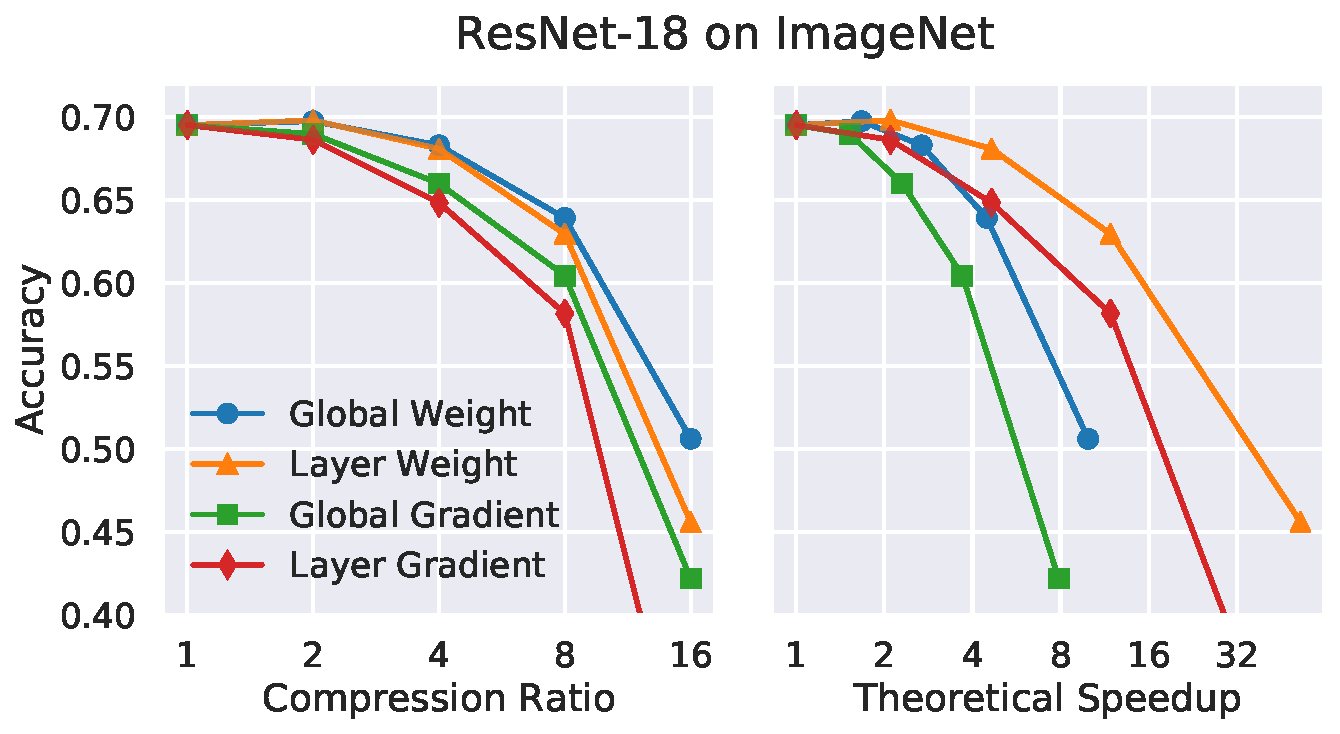
\includegraphics[width=\linewidth]{shrinkbench/ImageNet_flops}
% \vspace{-3mm}
\caption{Top 1 Accuracy for ResNet-18 on ImageNet for several compression ratios and their corresponding theoretical speedups.
%
Global methods give higher accuracy than Layerwise ones for a fixed model size, but the reverse is true for a fixed theoretical speedup.
}
\label{fig:ImageNet_flops}
\end{center}
\vspace*{-3mm}
\end{figure}

\vspace{-3mm}
\paragraph{Results Vary Across Models, Datasets, and Pruning Amounts}

Many methods report results on only a small number of datasets, models, amounts of pruning, and random seeds. If the relative performance of different methods tends to be constant across all of these variables, this may not be problematic. However, our results suggest that this performance is not constant.

Figure \ref{fig:sb_CIFAR10} shows the accuracy for various compression ratios for CIFAR-VGG \cite{vggCifarTorch} and ResNet-56 on CIFAR-10.
In general, Global methods are more accurate than Layerwise methods and Magnitude-based methods are more accurate than Gradient-based methods, with random performing worst of all.
However, if one were to look only at CIFAR-VGG for compression ratios smaller than 10, one could conclude that Global Gradient outperforms all other methods.
Similarly, while Global Gradient consistently outperforms Layerwise Magnitude on CIFAR-VGG, the opposite holds on ResNet-56 (i.e., the orange and green lines switch places).
% This is the opposite of the conclusion one would reach using ResNet-56, where that method is always outperformed by Global and Layerwise Magnitude Pruning.
%
% This shows the need to evaluate on a pruning method on various model and dataset combinations to ensure it is not architecture dependent.
%
% Similarly, this shows the need to report metrics for several compression rations to characterize the trade-off curve as pruning increases.
%

Moreover, we found that for some settings close to the drop-off point (such as Global Gradient, compression 16), different random seeds yielded significantly different results (0.88 vs 0.61 accuracy) due to the randomness in minibatch selection. This is illustrated by the large vertical error bar in the left subplot.

\begin{figure}[h]
\begin{center}
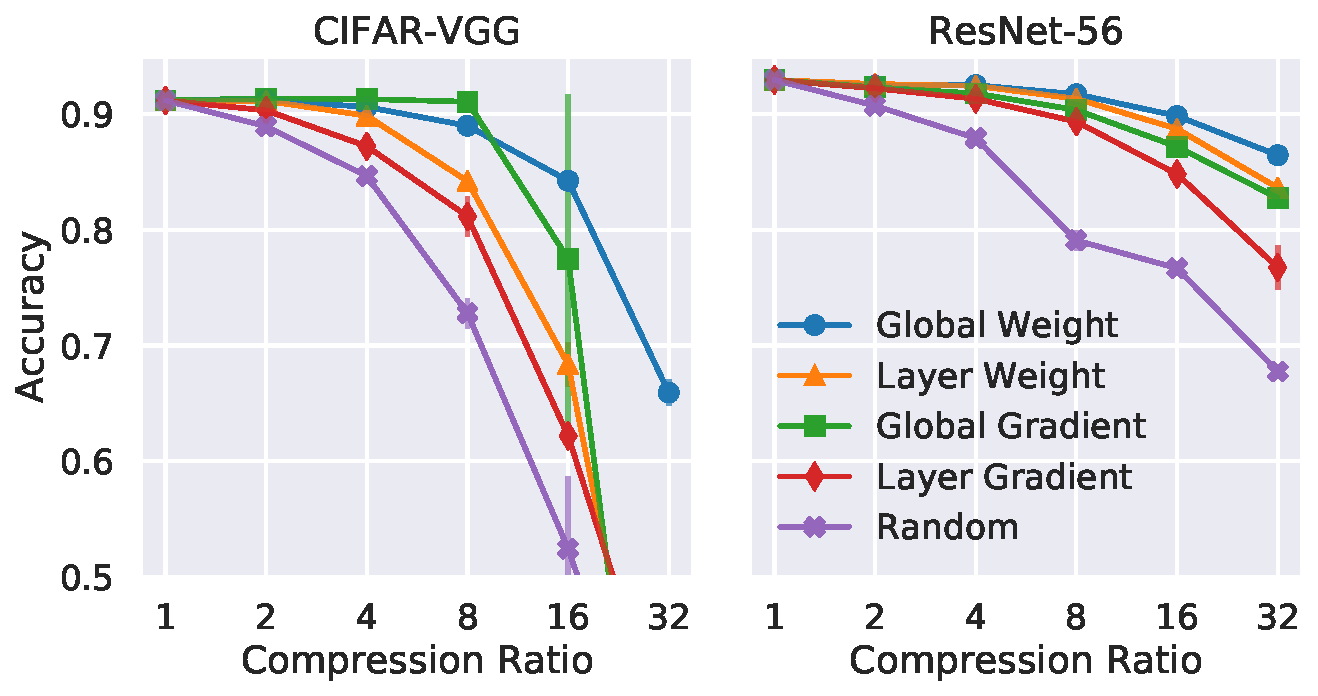
\includegraphics[width=\linewidth]{shrinkbench/CIFAR10_models}
% \vspace{-3mm}
\caption{Top 1 Accuracy on CIFAR-10 for several compression ratios.
%
 Global Gradient performs better than Global Magnitude for CIFAR-VGG on low compression ratios, but worse otherwise.
 Global Gradient is consistently better than Layerwise Magnitude on CIFAR-VGG, but consistently worse on ResNet-56.
 %
 % One standard deviation bars across three runs are included for all compression ratios greater than one.
}
\label{fig:sb_CIFAR10}
\end{center}
\end{figure}


% In absolute accuracy, Global strictly outperforms Layerwise Magnitude for both sets of pretrained weights.
% However, if we compare Layerwise Magnitude with pretrained weights A and Global with pretrained weights B, the previous conclusion could not be drawn.
%
% This is due to the fact that Layerwise with pretrained weights B has a smaller change in accuracy than Global with pretrained weights A for high compression ratios.
%
% This shows the need to use the same set of pretrained weights when comparing pruning methods since it can be a confounding factor.

\vspace{-4mm}
\paragraph{Using the Same Initial Model is Essential.}

As mentioned in Section~\ref{sec:confounding}, many methods are evaluated using different initial models with the same architecture. To assess whether beginning with a different model can skew the results, we created two different models and evaluated Global vs Layerwise Magnitude pruning on each with all other variables held constant.

To obtain the models, we trained two ResNet-56 networks using Adam until convergence with $\eta=10^{-3}$ and $\eta=10^{-4}$.
We'll refer to these pretrained weights as Weights A and Weights B, respectively.
% Figure \ref{fig:sb_resnet56_confounding} shows pruning results for these two sets of initial weights using each pruning method at several compression ratios.
%
As shown on the left side of Figure~\ref{fig:sb_resnet56_confounding}, the different methods appear better on different models. With Weights A, the methods yield similar absolute accuracies. With Weights B, however, the Global method is more accurate at higher compression ratios.

% We also see that the common practice of examining changes in accuracy is insufficient to correct for initial model as a confounder. In absolute accuracy, Global strictly outperforms Layerwise Magnitude Pruning for both sets of pretrained weights.
%
% However, if we compare Layerwise pruning with pretrained weights A and Global with pretrained weights B, the previous conclusion could not be drawn.
%
% This is due to the fact that Layerwise with pretrained weights B has a smaller change in accuracy than Global with pretrained weights A for high compression ratios.
%
% This shows the need to use the same set of pretrained weights when comparing pruning methods since it can be a confounding factor.

\begin{figure}[t]
\begin{center}
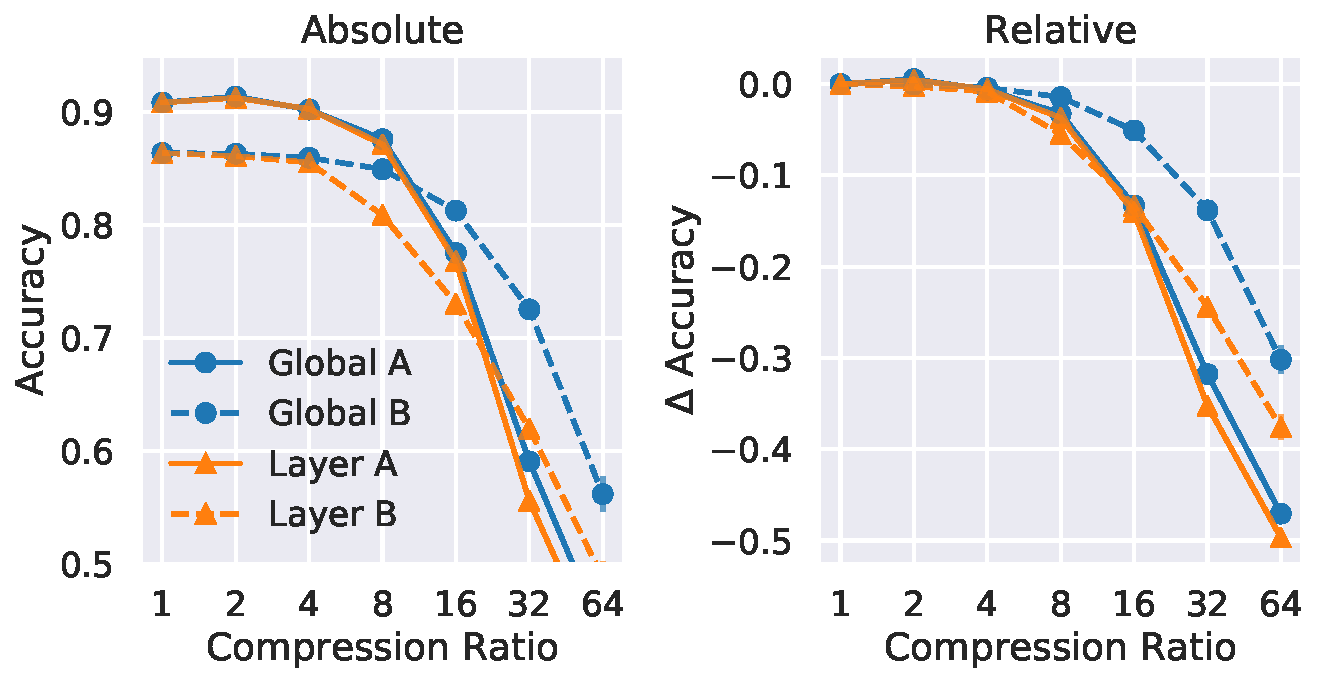
\includegraphics[width=\linewidth]{shrinkbench/confounding_resnet56}
% \vspace{-3mm}
\caption{Global and Layerwise Magnitude Pruning on two different ResNet-56 models.
%
% The starting models were obtained by training with Adam for 150 epochs with $\eta=10^{-3}$ (A) and $\eta=10^{-4}$ (B) respectively.
%
% One standard deviation bars across three runs are included for all compression ratios greater than one.
Even with all other variables held constant, different initial models yield different tradeoff curves. This may cause one method to erroneously appear better than another. Controlling for initial accuracy does not fix this. % problem.
% instead of raw accuracies, does not fix this problem.
}
\label{fig:sb_resnet56_confounding}
\end{center}
\end{figure}
We also found that the common practice of examining changes in accuracy is insufficient to correct for initial model as a confounder. Even when reporting changes, one pruning method can artificially appear better than another by virtue of beginning with a different model. We see this on the right side of Figure~\ref{fig:sb_resnet56_confounding}, where Layerwise Magnitude with Weights B appears to outperform Global Magnitude with Weights A, even though the former never outperforms the latter when initial model is held constant.

% Following \cite{google-state-of-sparsity}, we refrain from pruning

% \subsection{Design Goals}






%================================================================
\vspace{-1mm}
\section{Conclusion}
%================================================================

Considering the enormous interest in neural network pruning over the past decade, it seems natural to ask simple questions about the relative efficacy of different pruning techniques.
Although a few basic findings are shared across the literature, missing baselines and inconsistent experimental settings make it impossible to assess the state of the art or confidently compare the dozens of techniques proposed in recent years.
After carefully studying the literature and enumerating numerous areas of incomparability and confusion, we suggest concrete remedies in the form of a list of best practices and an open-source library---ShrinkBench---to help future research endeavors to produce the kinds of results that will harmonize the literature and make our motivating questions easier to answer. Furthermore, ShrinkBench results on various pruning techniques evidence the need for standardized experiments when evaluating neural network pruning methods.

%================================================================
\section*{Acknowledgements}
%================================================================

We thank Luigi Celona for providing the data used in \cite{luigi} and Vivienne Sze for helpful discussion. This research was supported by the Qualcomm Innovation Fellowship, the ``la Caixa'' Foundation Fellowship, Quanta Computer, and Wistron Corporation.

%``Benchmark Analysis of Representative Deep Neural Network Architectures.'' []

% ================================================================
% References
% ================================================================

% \IEEEtriggeratref{27} % trigger column break to make cols even
% \bibliographystyle{ACM-Reference-Format}
% \bibliographystyle{abbrev}
% \bibliographystyle{sysml2019}
\bibliographystyle{mlsys2020}
% \bibliography{prune,architectures,misc,understandDnn,classic,datasets,compress,science,metapapers,neuroscience}
\bibliography{combined}


\clearpage
\newpage  % so we can cut the pdf
\appendix



% TODO uncomment appendix after debug !!!!!!!!!!!!!!!!!!



\appendix


% ------------------------------------------------
\section{Corpus and Data Cleaning} \label{sec:corpus}
% ------------------------------------------------

% Before discussing the methodologies of our papers, we first discuss the methodology underlying our own claims. Because most of our conclusions follow directly from reading and tabulating the results in various neural network pruning papers, the bulk of our ``methodology'' is captured by the criteria used to select pruning papers.

We selected the \npapers papers used in our analysis in the following way. First, we conducted an ad hoc literature search, finding widely cited papers introducing pruning methods and identifying other pruning papers that cited them using Google Scholar. We then went through the conference proceedings from the past year's NeurIPS, ICML, CVPR, ECCV, and ICLR and added all relevant papers (though it is possible we had false dismissals if the title and abstract did not seem relevant to pruning). Finally, during the course of cataloging which papers compared to which others, we added to our corpus any pruning paper that at least one existing paper in our corpus purported to compare to. We included both published papers and unpublished ones of reasonable quality (typically on arXiv). Since we make strong claims about the lack of comparisons, we included in our corpus five papers whose methods technically do not meet our definition of pruning but are similar in spirit and compared to by various pruning papers.
In short, we included essentially every paper introducing a method of pruning neural networks that we could find, taking care to capture the full directed graph of papers and comparisons between them.
% TODO also manually go thru cvpr and eccv

% We analyze \npapers papers in total. These papers appear in the following venues:
% \begin{table}
% \begin{centering}
% \begin{tabular}{l|c}
% Venue & Number of Papers \\
% \hline
% arXiv & 20 \\
% NeurIPS & 16 \\
% ICLR & 12 \\
% CVPR & 9 \\
% ICML & 4 \\
% ECCV & 4 \\
% BMVC & 3 \\
% Nature Communications & 1 \\
% OpenReview & 1 \\
% IJCAI & 1 \\
% WACV & 1 \\
% AAAI & 1 \\
% CVPR Workshops & 1 \\
% MM & 1 \\
% Neurocomputing & 1 \\
% TPAMI & 1 \\
% IEEE Access & 1 \\
% ICASSP & 1 \\
% ICNN & 1 \\
% \label{tbl:venues}
% \end{tabular}
% \end{centering}
% % \vspace{2mm}
% \caption{Venues in which papers in our corpus appeared.}
% \end{table}

% To conduct our analysis, we normalized the reported

% In addition to choosing the set of papers to use, we also

% Define top venues.

% It is not always obvious what counts as a single method, even within one paper. For example, [uiuc-coreset]

% Define how we split up ``method'' for different papers, which is basically we called all their results one method unless something was an obvious straw man or there were two or more variations that reported values for the same amount of pruning (and therefore yielded two values at a given point on the tradeoff curve).

Because different papers report slightly different metrics, particularly with respect to model size, we converted reported results to a standard set of metrics whenever possible. For example, we converted reported Top-1 error rates to Top-1 accuracies, and fractions of parameters pruned to compression ratios. Note that it is not possible to convert between size metrics and speedup metrics, since the amount of computation associated with a given parameter can depend on the layer in which it resides (since convolutional filters are reused at many spatial positions). For simplicity and uniformity, we only consider self-reported results except where stated otherwise.

We also did not attempt to capture all reported metrics, but instead focused only on model size reduction and theoretical speedup, since 1) these are by far the most commonly reported and, 2) there is already a dearth of directly comparable numbers even for these common metrics. This is not entirely fair to methods designed to optimize other metrics, such as power consumption \cite{bayesian-compression, sze-energy-aware, learning-both, samsung-vbmf-tucker}, memory bandwidth usage \cite{extreme-net-compress, samsung-vbmf-tucker}, or fine-tuning time \cite{uiuc-coreset-pruning, pcas, sss, soft-filter-pruning}, and we consider this a limitation of our analysis.

% A further limitation is that,
Lastly, as a result of relying on reading of hundreds of pages of dense technical content, we are confident that we have made some number of isolated errors. We therefore welcome correction by email and refer the reader to the arXiv version of this paper for the most up-to-date revision.

% In certain cases, we break down results by whether papers were published in top-tier venues, as opposed to being published elsewhere or not at all. We define top venues as the top five relevant entries among Google Scholar's list of engineering and science venues with largest h5-indices \cite{scholarTopVenues}. The resulting venues are CVPR, NeurIPS, ICLR, ICML, and ECCV. While no list of ``top'' venues will be perfect or uncontroversial, this set accounts for the vast majority of published papers in our corpus. The exact set chosen is also of little consequence since there does not seem to be any difference between these and other papers with respect to the patterns we identify.

% All of the data we aggregated and used in a our analysis is available at TODO.

% Many of the quantitative results
% Describe results imputation. Note that one can't convert between compression and flops.

% Fact that we're only using self-reported results, and mention that this is what the vast majority of other papers do (or, more commonly, they don't say but kind of imply it).

% Some kind of background about pruning problem setup(s) and why you need particular (dset, architecture, xmetric, ymetric) tuples. Maybe define task = (dset, arch), and configuration = (dset, arch, xmetric, ymetric).

% Also mention something about how different authors care about different things (eg, energy efficiency, or at least one paper that brags about not having to fine-tune for as long as han2015). Mention that we can't capture all the nuance and that we don't try to question the validity of individual papers, except to the extent that they claim to be "state-of-the-art".

% A crucial aspect of the pruning task is that most methods can supply not just a single pruned network, but a family of networks with different sparsities. Which member of the family is returned depends on one or more tuning parameters (in addition to random variations). For example, methods that remove all but the largest-magnitude weights can choose how many weights to remove, and methods that apply L1-regularization to encourage sparsity can tune the L1 penalty. It is therefore crucial to compare pruning methods not just on the same dataset, architecture, and metrics, but also at similar operating points in their tradeoff curves. E.g., if one pruned 10\% of the weights based on magnitude and compared to pruning 50\% of the weights based on LASSO coefficients, the result would not be meaningful unless one method dominated in both efficiency and quality. % This means that a pruning method cannot be fully characterized by a single network it has produced, but must instead be evaluated based on the \textit{tradeoff curve} it supplies for a given dataset, model, efficiency metric, and quality metric. This is similar to the need for precision-recall curves, Precision at K, and/or Recall at K curves for search and ranking algorithms. % , or the Receiver Operating Characteristic (ROC) curve for risk stratification algorithms. % However, while some of these other curves have widely-accepted summary statistics such as mean average precision (mAP) or Area Under the Curve (AUC), there is no such statistic for arbitrary tradeoff curves. % AUC could perhaps be adapted, but only with great difficulty since the efficiency metric is either unbounded

%!TEX root = doc.tex
%!TEX output_directory = aux

% ------------------------------------------------
\section{Checklist for Evaluating a Pruning Method} \label{apx:recommendations}
% ------------------------------------------------

\noindent For any pruning technique proposed, check if:
\begin{itemize}
\item It is contextualized with respect to magnitude pruning, recently-published pruning techniques, and pruning techniques proposed prior to the 2010s.
\item The pruning algorithm, constituent subroutines (e.g., score, pruning, and fine-tuning functions), and hyperparameters are presented in enough detail for a reader to reimplement and match the results in the paper.
\item All claims about the technique are appropriately restricted to only the experiments presented (e.g., CIFAR-10, ResNets, image classification tasks, etc.).
\item There is a link to downloadable source code.
\end{itemize}

\noindent For all experiments, check if you include:
\begin{itemize}
\item A detailed description of the architecture with hyperparameters in enough detail to for a reader to reimplement it and train it to the same performance reported in the paper.
\item If the architecture is not novel: a citation for the architecture/hyperparameters and a description of any differences in architecture, hyperparameters, or performance in this paper.
\item A detailed description of the dataset hyperparameters (e.g., batch size and augmentation regime) in enough detail for a reader to reimplement it.
% \item A list of other prior pruning papers that include the same architecture, dataset, and hyperparameters.
\item A description of the library and hardware used.
\end{itemize}

\noindent For all results, check if:
\begin{itemize}
\item Data is presented across a range of compression ratios, including extreme compression ratios at which the accuracy of the pruned network declines substantially.
\item Data specifies the raw accuracy of the network at each point.
\item Data includes multiple runs with separate initializations and random seeds.
\item Data includes clearly defined error bars and a measure of central tendency (e.g., mean) and variation (e.g., standard deviation).
\item Data includes FLOP-counts if the paper makes arguments about efficiency and performance due to pruning.
\end{itemize}

\noindent For all pruning results presented, check if there is a comparison to:
\begin{itemize}
\item A random pruning baseline.
    \begin{itemize}
    \item A global random pruning baseline.
    \item A random pruning baseline with the same layerwise pruning proportions as the proposed technique.
    \end{itemize}
\item A magnitude pruning baseline.
    \begin{itemize}
    \item A global or uniform layerwise proportion magnitude pruning baseline.
    \item A magnitude pruning baseline with the same layerwise pruning proportions as the proposed technique.
    \end{itemize}
\item Other relevant state-of-the-art techniques, including:
    \begin{itemize}
    \item A description of how the comparisons were produced (data taken from paper, reimplementation, or reuse of code from the paper) and any differences or uncertainties between this setting and the setting used in the main experiments.
    \end{itemize}
\end{itemize}

%!TEX root = doc.tex
%!TEX output_directory = aux

\section{Experimental Setup} \label{apx:exp}

For reproducibility purposes, \SB{} fixes random seeds for all the dependencies (\texttt{PyTorch}, \texttt{NumPy}, \texttt{Python}).


\subsection{Pruning Methods}

For the reported experiments, we did not prune the classifier layer preceding the softmax.
%
\SB{} supports pruning said layer as an option to all proposed pruning strategies.
%
For both Global and Layerwise Gradient Magnitude Pruning a single minibatch is used to compute the gradients for the pruning.
%
Three independent runs using different random seeds were performed for every CIFAR10 experiment.
%
We found some variance across methods that relied on randomness, such as random pruning or gradient based methods that use a sampled minibatch to compute the gradients with respect to the weights.


\subsection{Finetuning Setup}

Pruning was performed from the pretrained weights and fixed from there forwards.
%
% Reported values are always for the validation set.
%
Early stopping is implemented during finetuning.
%
Thus if the validation accuracy repeatedly decreases after some point we stop the finetuning process to prevent overfitting.
%
% We did not perform any hyperparameter search across finetuning hyperparameters.

All reported CIFAR10 experiments used the following finetuning setup:
\begin{itemize}[leftmargin=4mm]
    \itemsep-2pt
    \vspace{-2mm}
    \item Batch size: 64
    \item Epochs: 30
    \item Optimizer: Adam
    \item Initial Learning Rate: $3 \times 10^{-4}$
    \item Learning rate schedule: Fixed
\end{itemize}
%
All reported ImageNet experiments used the following finetuning setup
\begin{itemize}[leftmargin=4mm]
    \itemsep-2pt
    \vspace{-2mm}
    \item Batch size: 256
    \item Epochs: 20
    \item Optimizer: SGD with Nesterov Momentum (0.9)
    \item Initial Learning Rate: $1 \times 10^{-3}$
    \item Learning rate schedule: Fixed
\end{itemize}

%!TEX root = doc.tex
%!TEX output_directory = aux

\section{Additional Results} \label{apx:res}


Here we include the entire set of results obtained with \SB.
%
For CIFAR10, results are included for CIFAR-VGG, ResNet-20, ResNet-56 and ResNet-110. Standard deviations across three different random runs are plotted as error bars.
%
For ImageNet, results are reported for ResNet-18.

\clearpage

\begin{figure*}
\begin{minipage}[b]{.45\textwidth}
\centering
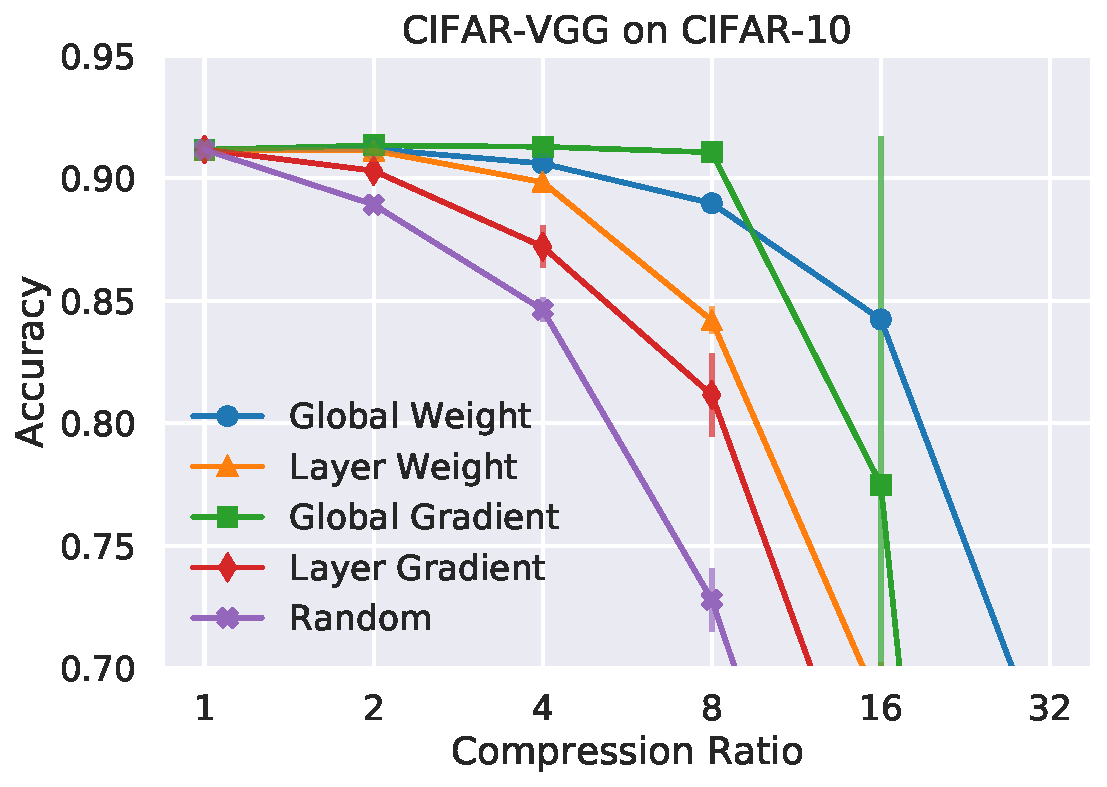
\includegraphics[width=\linewidth]{shrinkbench/VGG-CIFAR_CIFAR10_comp}
\captionof{figure}{Accuracy for several levels of compression for CIFAR-VGG on CIFAR-10}
\end{minipage}
\hfill
\begin{minipage}[b]{.45\textwidth}
\centering
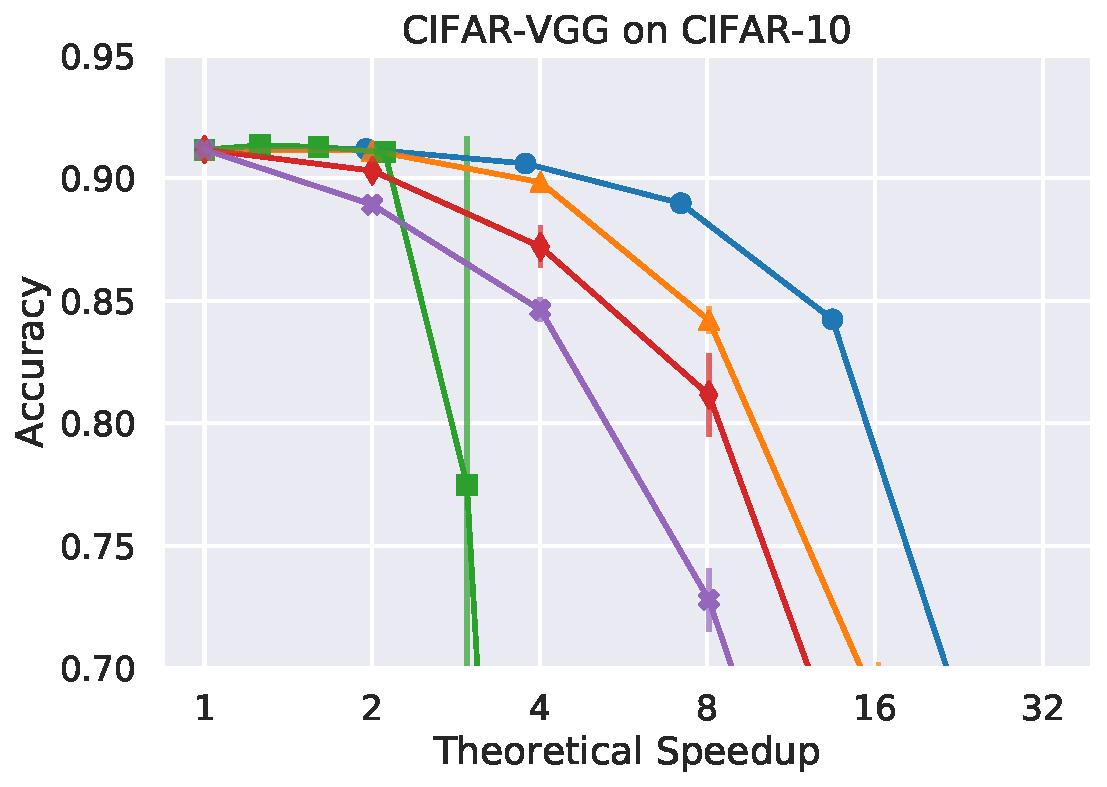
\includegraphics[width=\linewidth]{shrinkbench/VGG-CIFAR_CIFAR10_flops}
\caption{Accuracy vs theoretical speedup for CIFAR-VGG on CIFAR-10}
\end{minipage}
\end{figure*}


\begin{figure*}
\begin{minipage}[b]{.45\textwidth}
\centering
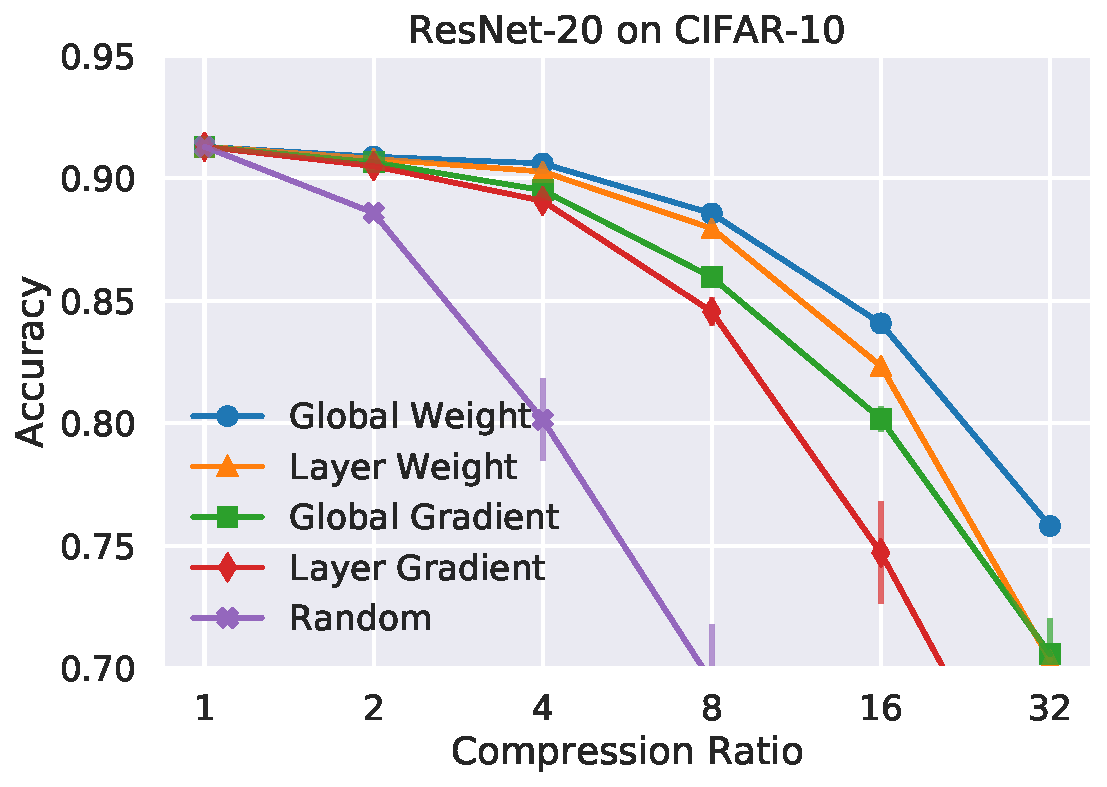
\includegraphics[width=\linewidth]{shrinkbench/resnet20_CIFAR10_comp}
\caption{Accuracy for several levels of compression for ResNet-20 on CIFAR-10}
\end{minipage}
\hfill
\begin{minipage}[b]{.45\textwidth}
\centering
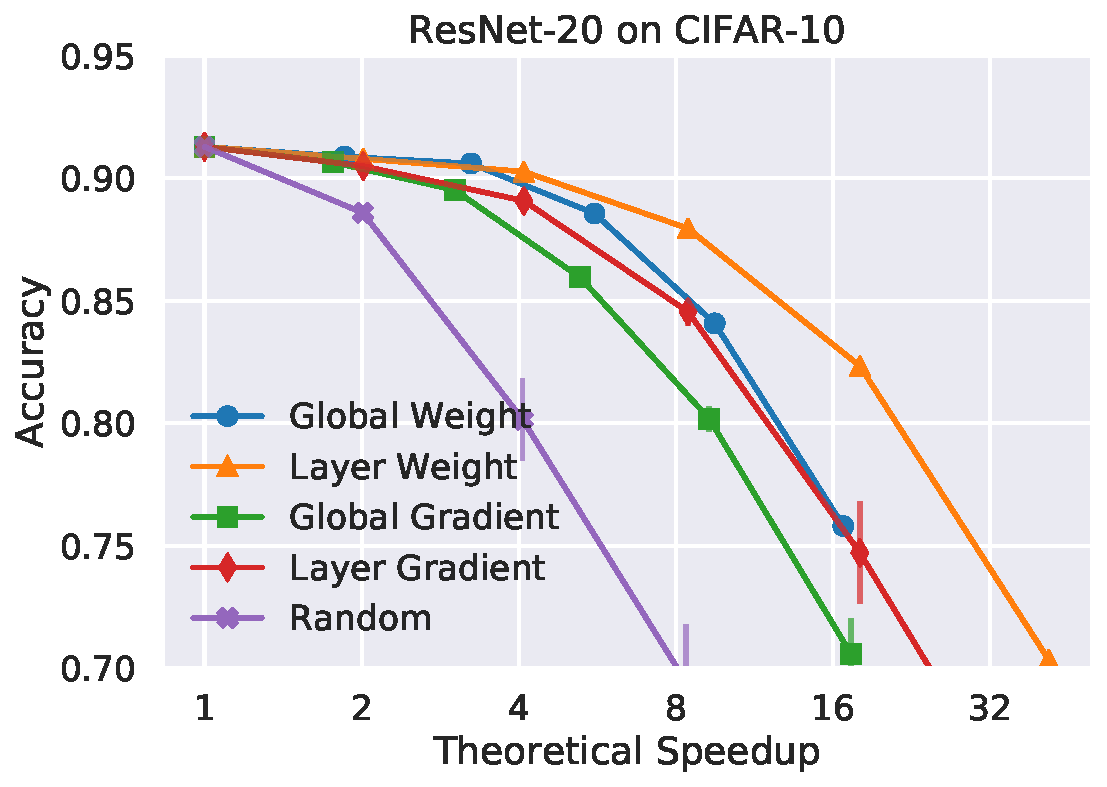
\includegraphics[width=\linewidth]{shrinkbench/resnet20_CIFAR10_flops}
\caption{Accuracy vs theoretical speedup for ResNet-20 on CIFAR-10}
\end{minipage}
\end{figure*}

\begin{figure*}
\begin{minipage}[b]{.45\textwidth}
\centering
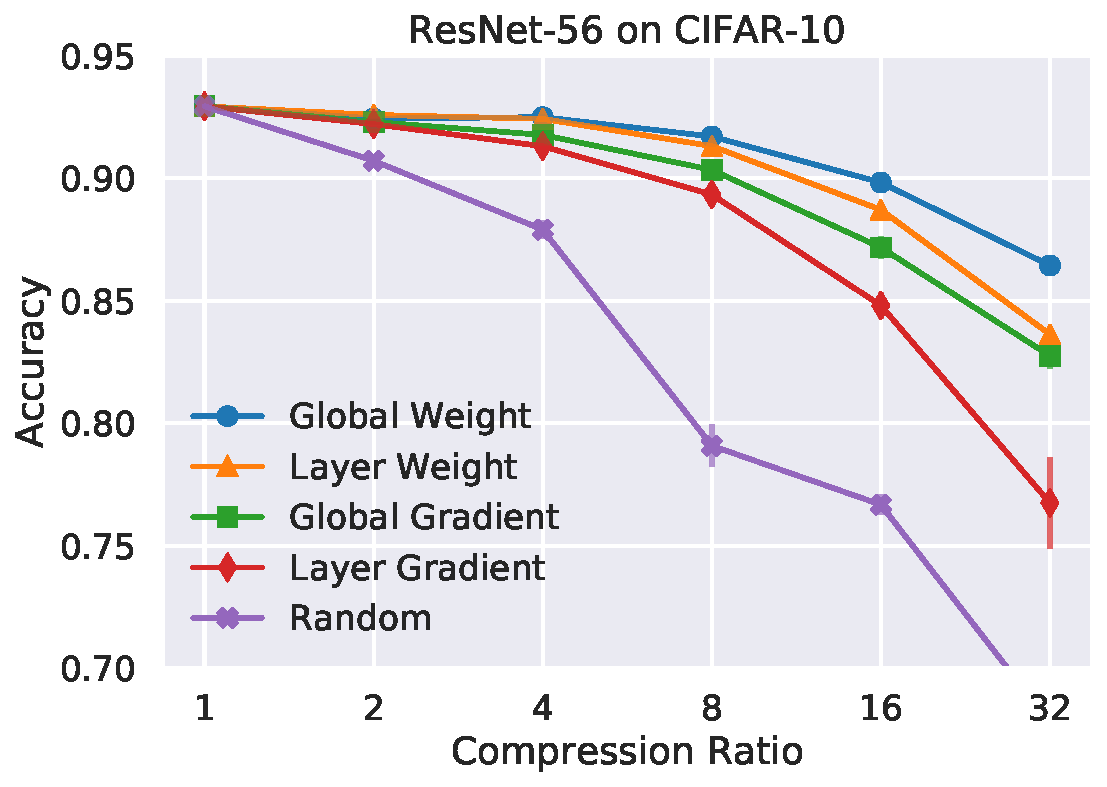
\includegraphics[width=\linewidth]{shrinkbench/resnet56_CIFAR10_comp}
\captionof{figure}{Accuracy for several levels of compression for ResNet-56 on CIFAR-10}
\end{minipage}
\hfill
\begin{minipage}[b]{.45\textwidth}
\centering
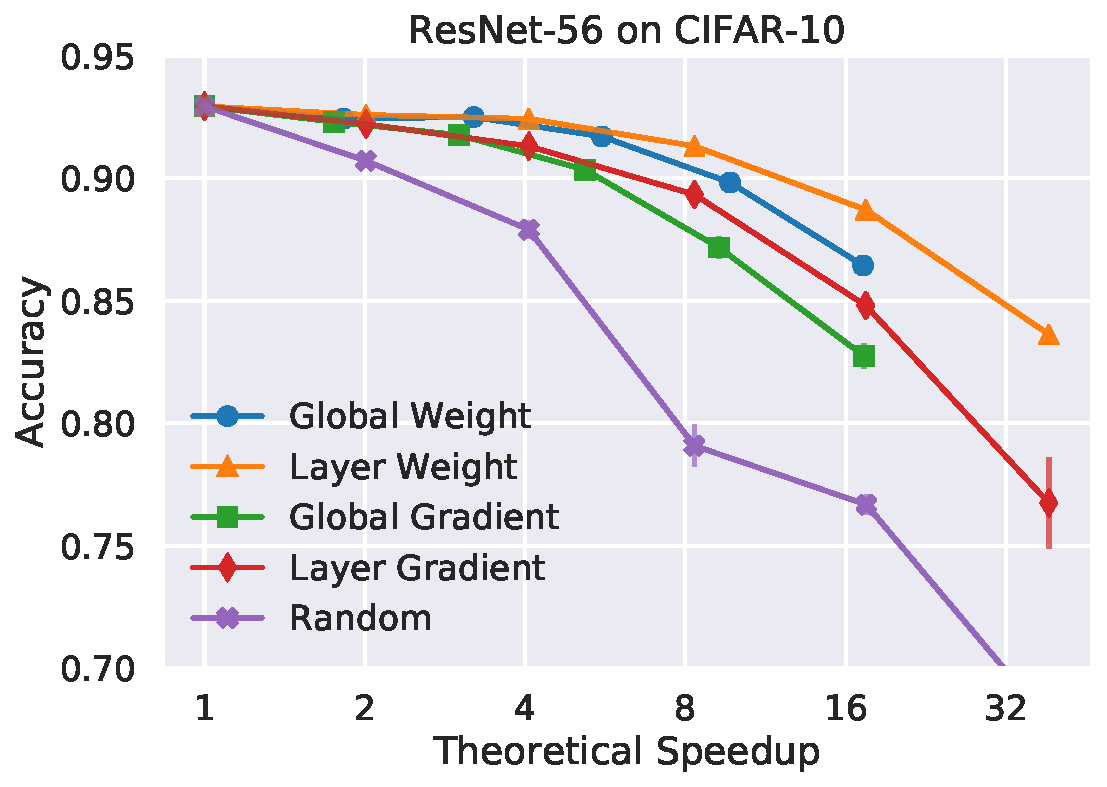
\includegraphics[width=\linewidth]{shrinkbench/resnet56_CIFAR10_flops}
\caption{Accuracy vs theoretical speedup for ResNet-56 on CIFAR-10}
\end{minipage}
\end{figure*}


% NEWPAGE



\begin{figure*}
\begin{minipage}[b]{.45\textwidth}
\centering
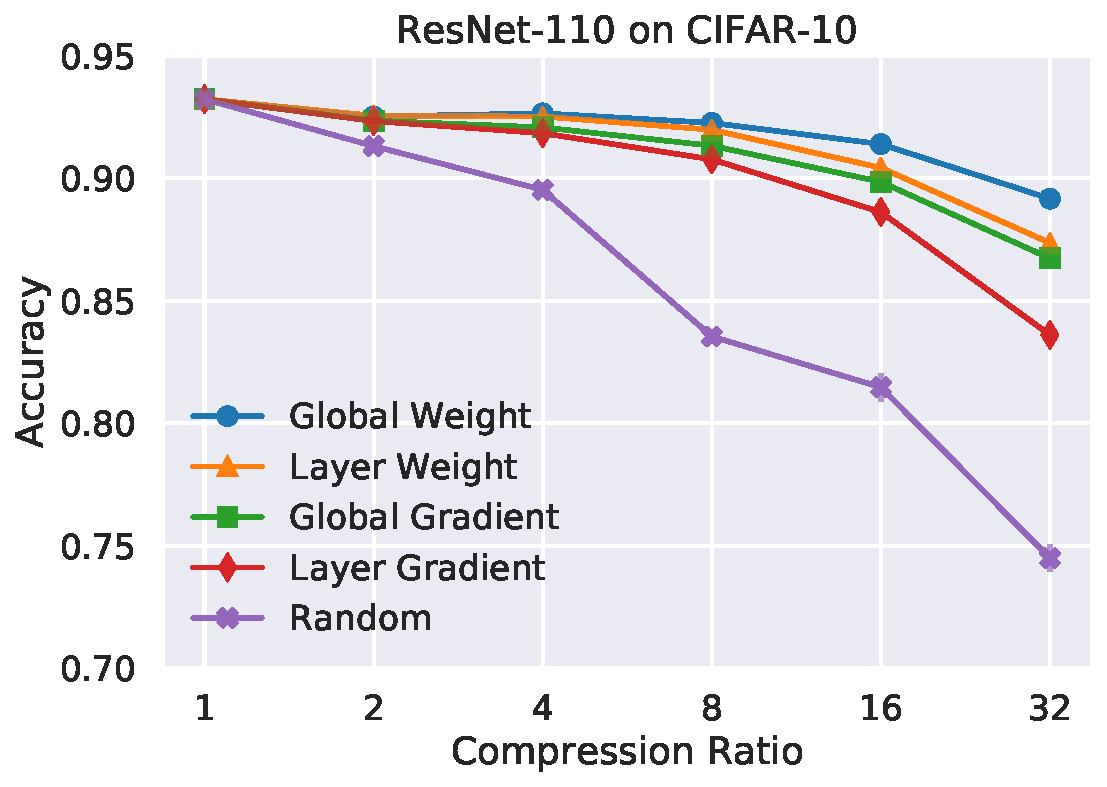
\includegraphics[width=\linewidth]{shrinkbench/resnet110_CIFAR10_comp}
\caption{Accuracy for several levels of compression for ResNet-110 on CIFAR-10}
\end{minipage}
\hfill
\begin{minipage}[b]{.45\textwidth}
\centering
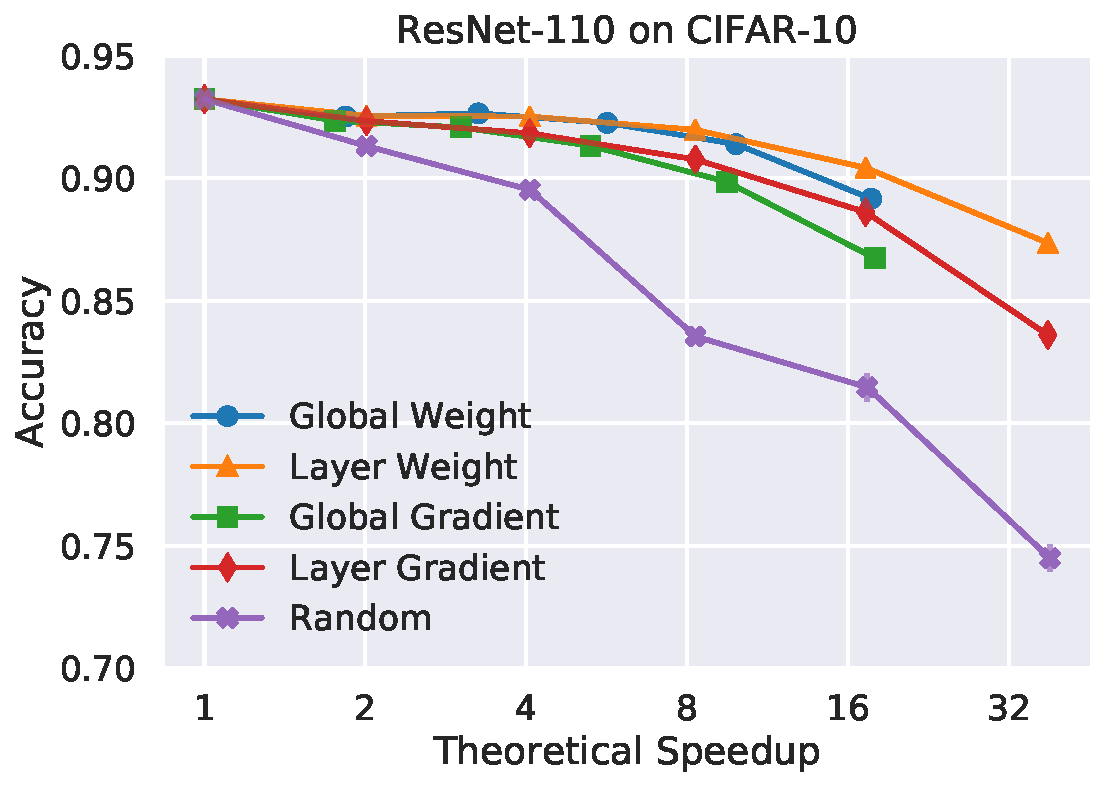
\includegraphics[width=\linewidth]{shrinkbench/resnet110_CIFAR10_flops}
\caption{Accuracy vs theoretical speedup for ResNet-110 on CIFAR-10}
\end{minipage}
\end{figure*}



\begin{figure*}
\begin{minipage}[b]{.45\textwidth}
\centering
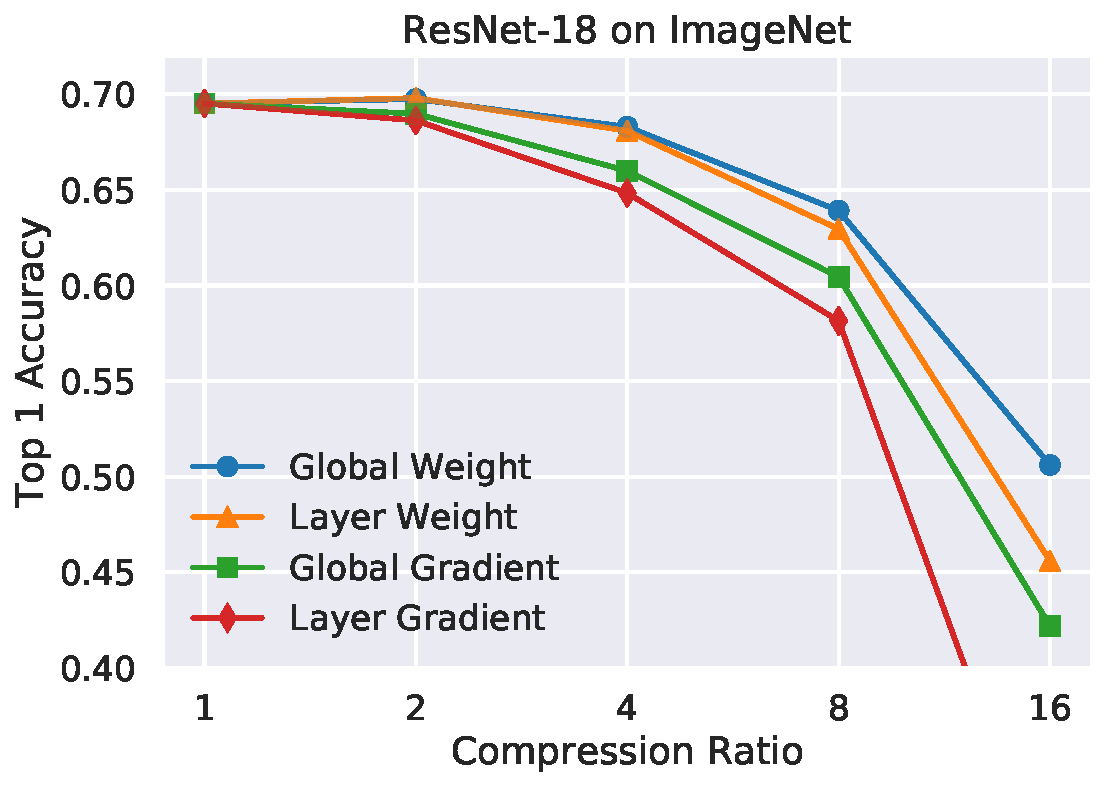
\includegraphics[width=\linewidth]{shrinkbench/resnet18_ImageNet_comp}
\caption{Accuracy for several levels of compression for ResNet-18 on ImageNet}
\end{minipage}
\hfill
\begin{minipage}[b]{.45\textwidth}
\centering
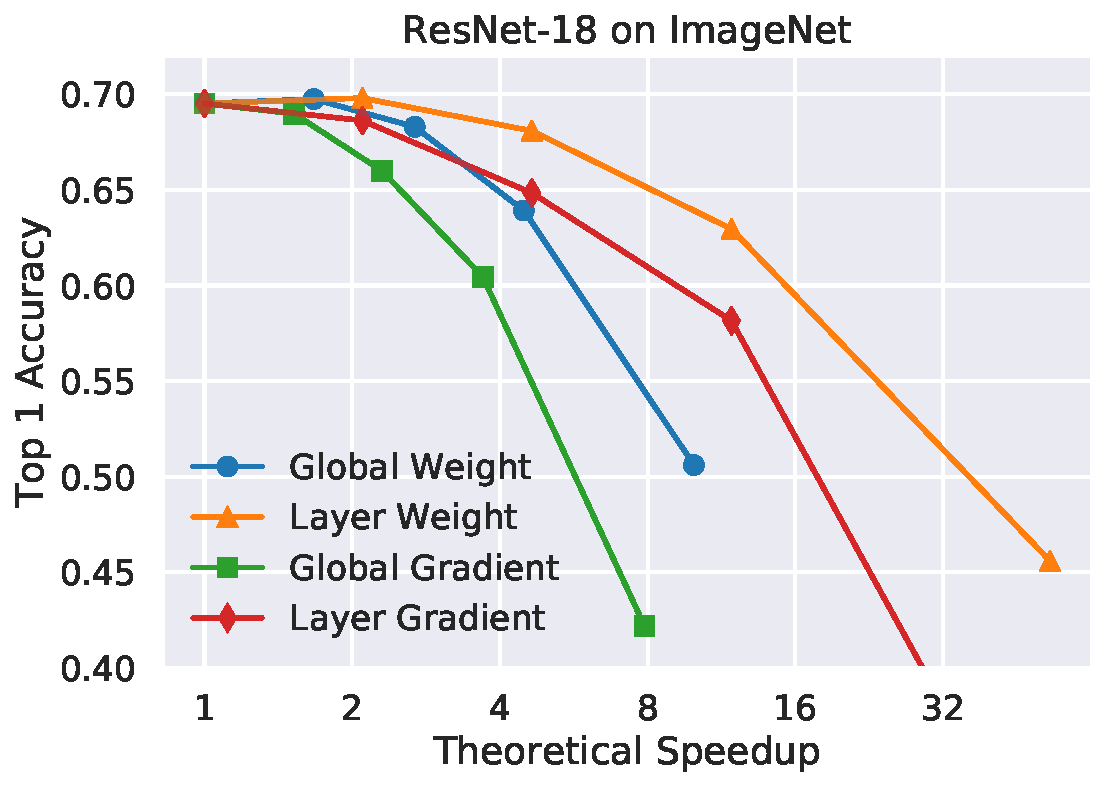
\includegraphics[width=\linewidth]{shrinkbench/resnet18_ImageNet_flops}
\caption{Accuracy vs theoretical speedup for ResNet-18 on ImageNet}
\end{minipage}
\end{figure*}



\end{document}
